%
% main.tex -- Paper zum Thema Audio-Kompression mit Daubechies-Wavelets
%
% (c) 2019 Hochschule Rapperswil
%
\chapter{Audio-Komprimierung mit Daubechies Wavelets\label{chapter:compress}}
\lhead{Audio-Komprimierung mit Daubechies Wavelets}
\begin{refsection}
\chapterauthor{Julian Bärtschi}

\section{Audio-Komprimierung}
\rhead{Vorwort}
Die Menge an produzierten Daten nimmt jährlich rasant zu.
Immer höher aufgelöste Bild-, Video- und Audiodaten spielen dabei eine zentrale Rolle.
Um den Berg an Daten im Griff zu behalten, ist Datenkomprimierung (lat.~comprimere, `zusammendrücken') unerlässlich. 

Das Ziel der Datenkomprimierung ist, die vorhandenen Daten so zu verdichten, dass der Speicherbedarf möglichst reduziert werden kann.
Es sollen für die Speicherung, wie auch für die Übertragung der Daten möglichst wenig Ressourcen benötigt werden.

Diese Arbeit wird auf Audiodaten beschränkt.
Dabei ist das Ziel nicht etwa die Entwicklung eines Kompressionsalgorithmus sondern das Aufzeigen von Möglichkeiten der Komprimierung mit Hilfe von Wavelets.
Des Weiteren steht eine exakte Rekonstruktion nicht im Vordergrund, jedoch soll für den Hörer möglichst keinen Unterschied zum Original wahrnehmbar sein.

\subsection{Verlustfreie Komprimierung}
Bei der verlustfreien Komprimierung wird gewährleistet, dass die Originaldaten exakt aus den komprimierten Daten wiederhergestellt werden können.
Es wird die Tatsache ausgenutzt, dass gewisse Daten redundant vorkommen. 
Deshalb spricht man auch von Redundanzreduktion.

Verlustfreie Komprimierung findet breite Anwendung.
Insbesondere bei Datenarchivierung sollen die Originaldaten exakt erhalten bleiben und darum wird häufig eine solche Kompressionstechnik verwendet.
Namhafte Beispiele von verlustfreier Komprimierung sind beispielsweise das ZIP-Dateiformat, die Portable Network Graphics (PNG) oder im Bezug auf Audiodaten der Free Lossless Audio Codec (FLAC).
Beispielsweise kann mit dem FLAC-8 der Speicherplatzbedarf auf unter 66 Prozent der Originaldatei reduziert werden, ohne dabei Informationen zu verlieren \cite{wikipedia:flac}.

\subsection{Verlustbehaftete Komprimierung}
Bei der verlustbehafteten Komprimierung soll nur der nötige Teil der Originaldaten erhalten bleiben.
Somit ist es möglich, den benötigten Speicherplatz auf ein Minimum zu reduzieren.
Das hat jedoch zur Folge, dass die Originaldaten nicht mehr exakt wiederhergestellt werden können. 
Somit ist diese Form der Komprimierung nicht wieder umkehrbar.
Man kann unnötige Daten entfernen und somit die Datenmenge reduzieren.
Deshalb spricht man auch von Irrelevanzreduktion.
Die verlustbehaftete Komprimierung wird insbesondere für Audio- und Video-Daten häufig verwendent.
Um zu entscheiden, welche Teile wichtig und welche entbehrlich sind, wird auf die menschliche Wahrnehmung geachtet.
Weil die menschliche Sinneswahrnehmung nicht alle Frequenzen und Töne gleich gut aufnimmt, können gewisse Bereiche weggelassen werden.
Mehr dazu im folgenden Kapitel.

Mit der verlustbehafteten Kompression können sehr hohe Kompressionsraten erreicht werden, welche aber stets mit einer Qualitätseinbusse kommen.
Diesen Abtausch von hoher Kompression mit schlechter Qualität gilt es abzuschätzen.

\section{Psychoakustik}
\rhead{Psychoakustik}
\label{chapter:Psychoakustik}
Das menschliche Gehör verarbeitet Schallwellen nicht einfach wie ein Mikrofon.
Um ein Schallereignis zu beurteilen haben Psychoakustiker eine Vielzahl an Parametern identifiziert, beispielsweise Lautheit und Schärfe, auf welche in dieser Arbeit aber nicht weiter eingegangen wird.

\begin{figure}
	\centering
	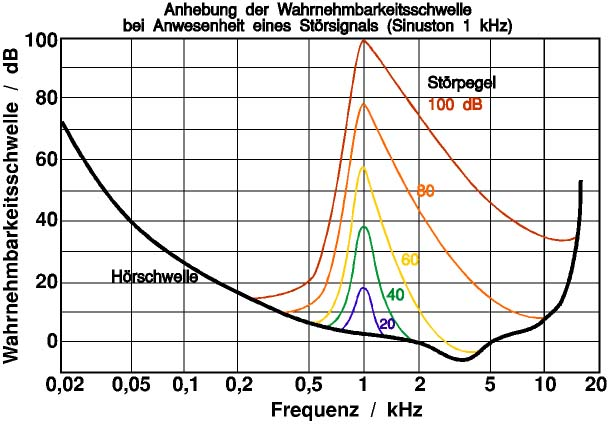
\includegraphics[width=0.6\linewidth]{papers/compress/Bilder/Akustik_Mithoerschwelle2}
	\caption{Wahrnehmbarkeit von Schallsignalen bei Anwesenheit von Störsignalen \cite{skript:Akustik2}}
	\label{fig:Wahrnehmbarkeitsschwelle}
\end{figure}

In \autoref{fig:Wahrnehmbarkeitsschwelle} dargestellt ist ein Modell der Wahrnehmbarkeitsschwelle des menschlichen Gehörs.
Dabei wurde die Lautstärke von $0\,\text{dB}$ gerade an dem Ort festgelegt, an dem ein $2\,\text{kHz}$ Ton gerade hörbar wird.
Ausserdem entspricht eine Signalverdoppelung gerade einer Erhöhung um $6\,\text{dB}$. 
Bei einem vorhandenen Störsignal, hier $1\,\text{kHz}$, wird diese Schwelle merklich angehoben.
Auch zeitlich werden leise Töne kurz vor und nach einem lauten Ton verdeckt \cite{wikipedia:Psychoakustik}.

Nun folgt die Überlegung, dass jene Daten die nicht wahrnehmbar sind (unter der Schwelle) redundant sind und weggelassen werden können.
Dies suggeriert grosses Potential für die verlustbehaftete Komprimierung.

\section{Warum Daubechies-Wavelets?}
\rhead{Warum Daubechies-Wavelets?}
\label{chapter:daubechies}
Um ein Signal möglichst gut zu analysieren, muss zuerst ein geeignetes Wavelet gewählt werden.
Die in \autoref{chapter:kompakt} vorgestellten Daubechies-Wavelets besitzen sehr nützliche Eigenschaften.
Um die folgenden Abschnitte etwas übersichtlicher zu gestalten wird der Term `Daubechies-Wavelet $N$-ter Ordnung' nun mit `dbN' abgekürzt.
Das Haar-Wavelet (db1) hat die Eigenschaft, dass es verschwindet, solange nicht mindestens ein lineares Signal analysiert wird.
Für das db2 gilt dasselbe mit quadratischen Funktionen. 
Die Ordnung des Wavelets nimmt also zusammen mit der Ordnung des analysierten Signals zu.
\begin{figure}
	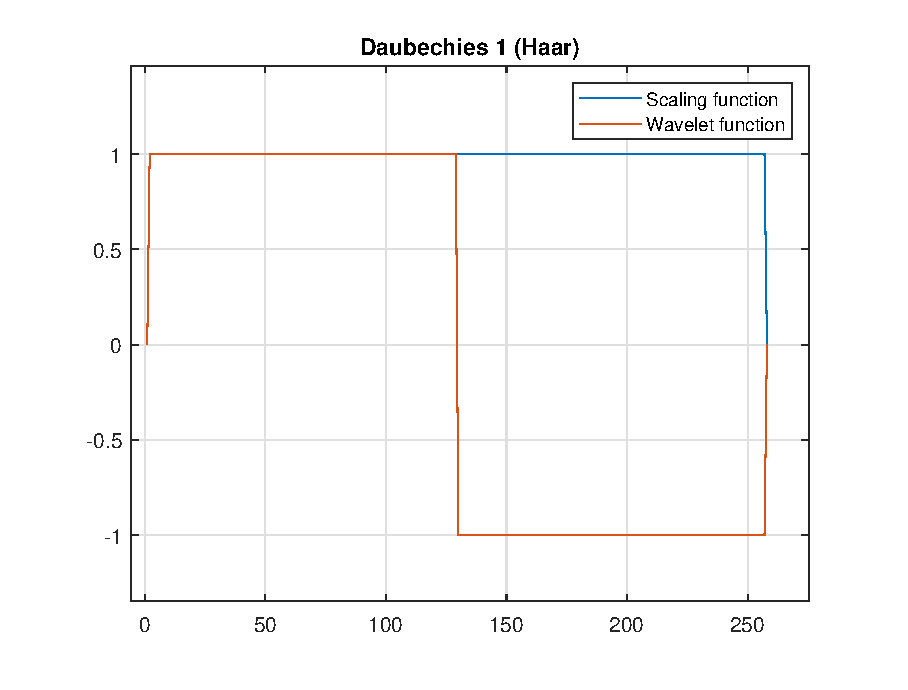
\includegraphics[width=0.5\linewidth]{papers/compress/Bilder/db1}
	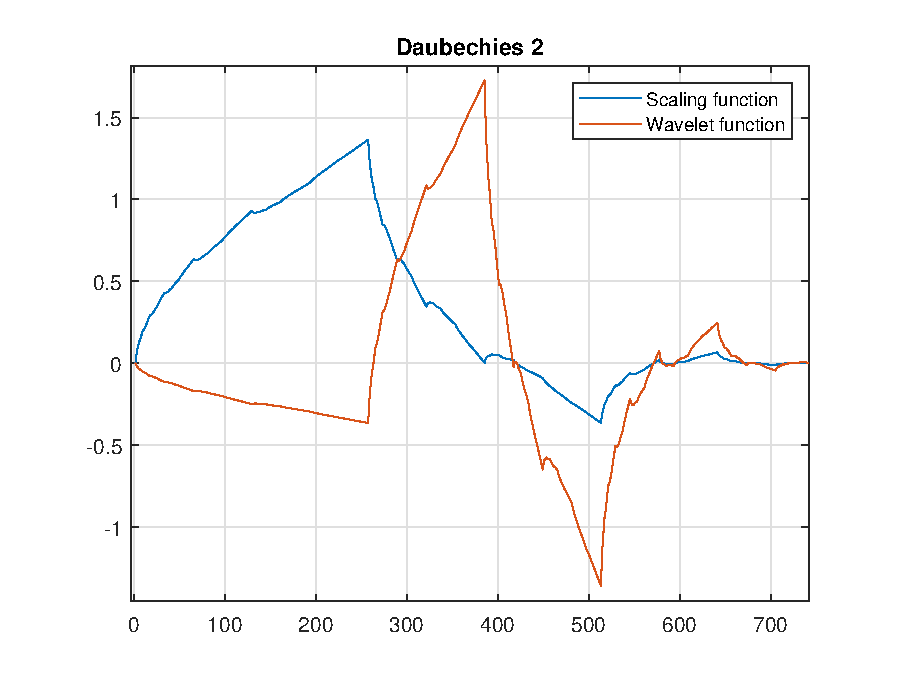
\includegraphics[width=0.5\linewidth]{papers/compress/Bilder/db2}
	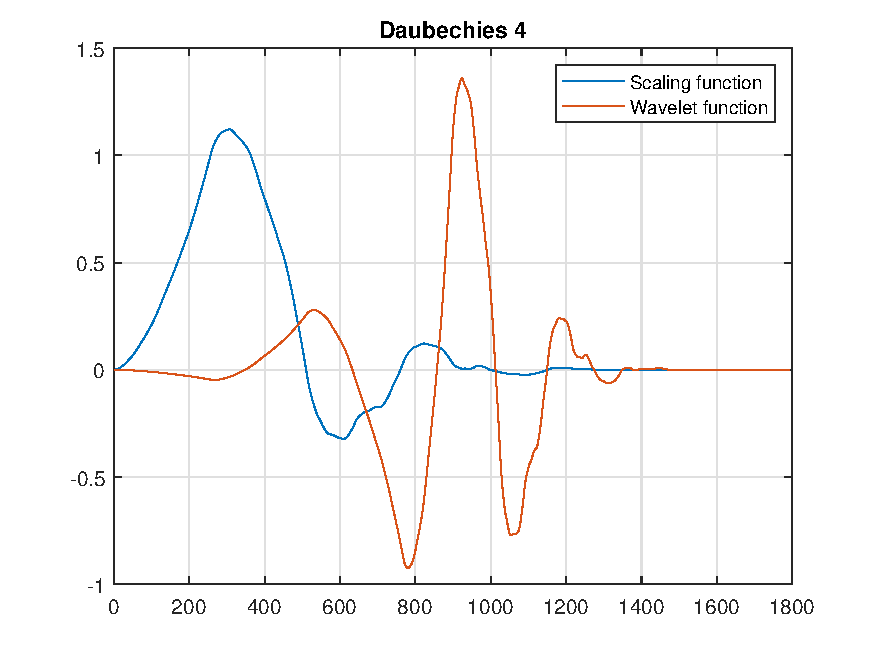
\includegraphics[width=0.5\linewidth]{papers/compress/Bilder/db4}
	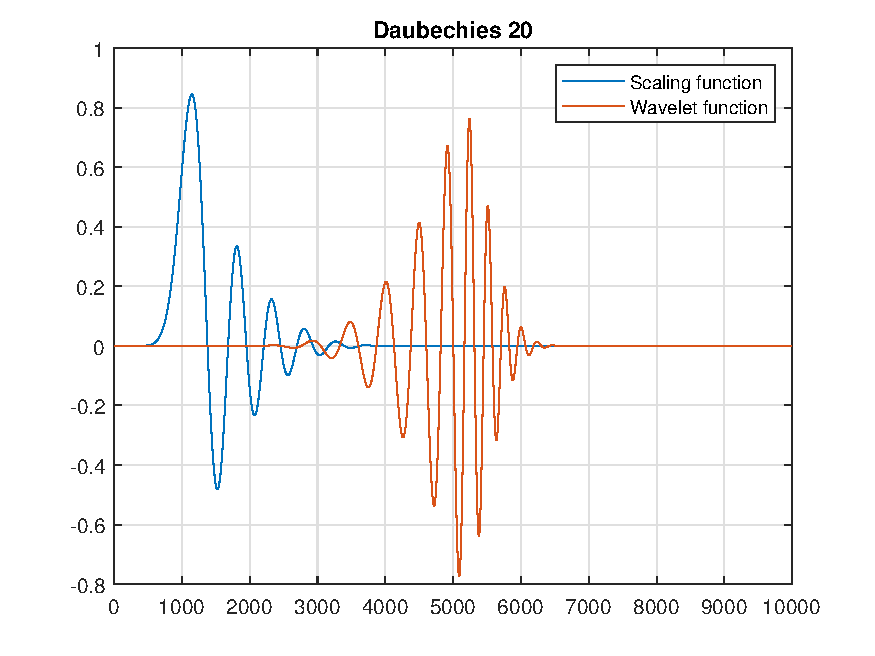
\includegraphics[width=0.5\linewidth]{papers/compress/Bilder/db20}
	\label{fig:dbN}
	\caption{Daubechies-Wavelets unterschiedlicher Ordnungen.}
\end{figure}

Da im Audiobereich sehr steile Signale möglich sind, können Daubechies-Wavelets einer hohen Ordnung sehr gute Werte liefern.
Das bedeutet zum einen, dass sehr unterschiedliche Signale damit abgetastet werden können und zum anderen, dass die Wavelettransformationen genau Null geben, wenn sie auf Signale der tieferen Ordnung angewendet werden.
Wenn man die Wahrnehmbarkeitsschwelle von \autoref{fig:Wahrnehmbarkeitsschwelle} betrachtet, liegt es nahe, dass eine Folge von Nullwerten oder auch Werte in der Nähe von Null nicht gespeichert werden müssen.
Somit bilden die Daubechies-Wavelets eine gute Grundlage für diese Anwendung.
Für diese Arbeit wurden hauptsächlich die beiden Wavelets `db4' sowie `db20' verwendet.

\section{Anwendung}
\rhead{Anwendung}
Für die Analyse von Audiodaten wird eine Multiskalenanalyse, wie in \autoref{chapter:msa} beschrieben, durchgeführt.
Die Anzahl \textit{n} der Levels dieser Analyse wird anhand der Länge \textit{l} des Signals mit
\begin{equation}
\textit{n} = \log_2{\textit{l}}
\end{equation}
berechnet.

\subsection{Das Prinzip}
Als Beispiel wird die Analyse einer gewöhnlichen Sägezahnschwingung in \autoref{fig:sawtooth} dargestellt.
\begin{figure}
	\centering
	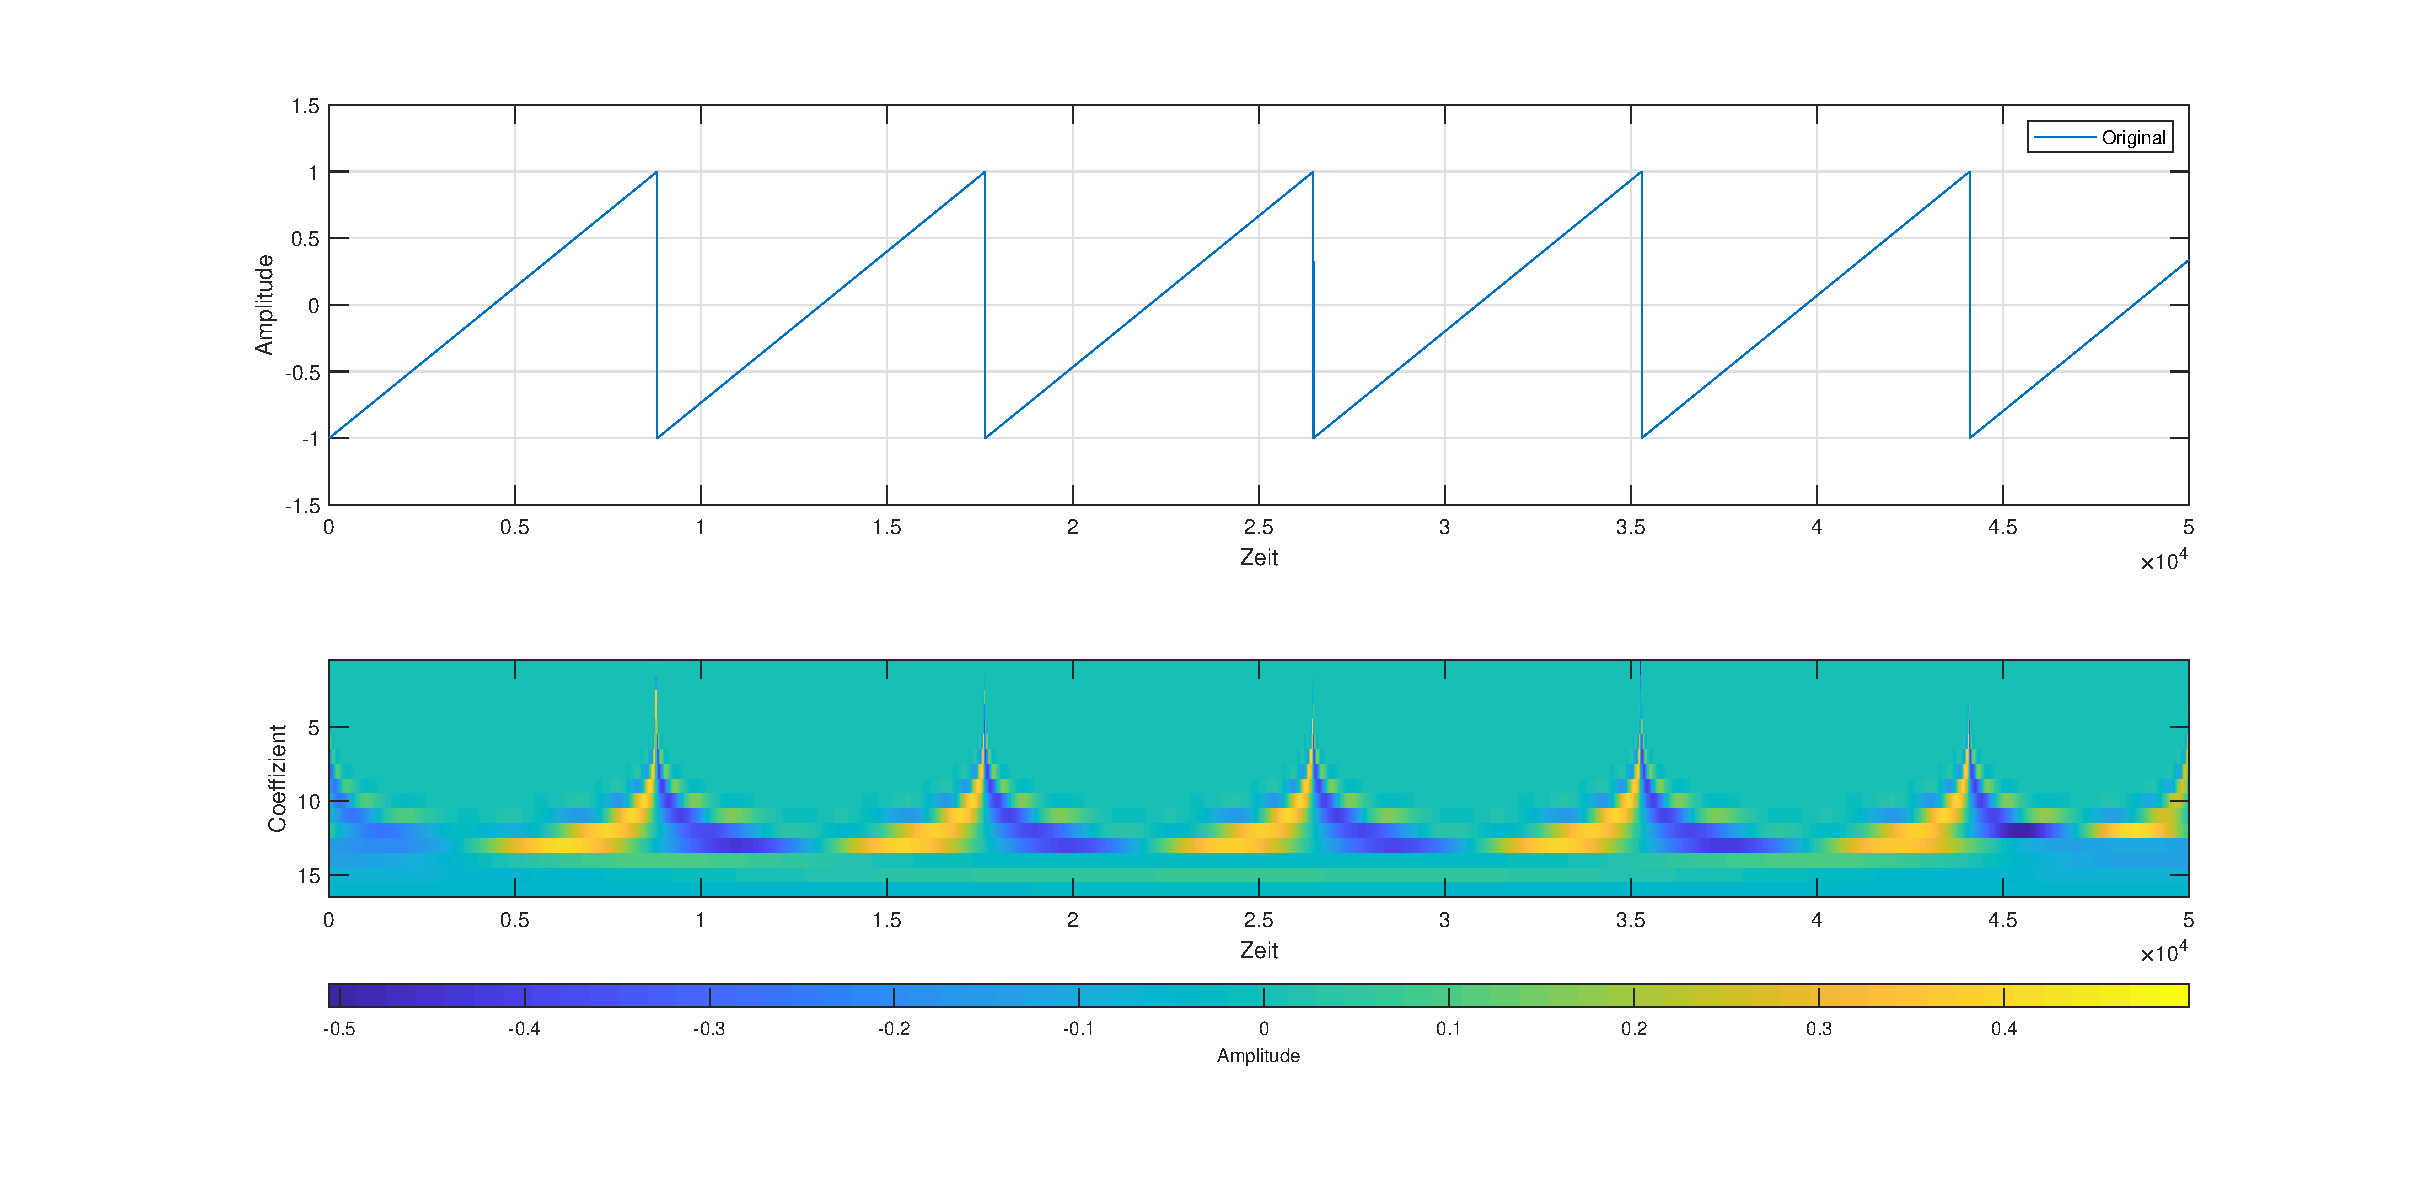
\includegraphics[width=\linewidth]{papers/compress/Bilder/sawtooth}
	\caption{Multiskalenanalyse einer Sägezahnschwingung}
	\label{fig:sawtooth}
\end{figure}
Während dem linearen Anstieg des Sägezahns ist erkennbar, wie die Multiskalenanalyse über alle Skalierungslevels gleich Null ist.
In diesem Beispiel wurde ein db4 verwendet.
Sobald diese unterschiedlich skalierten Wavelets in einen Bereich gelangen, bei dem sich die Amplitude stark ändert, ist ein Wert ungleich Null erkennbar.
Für die sehr klein skalierten Wavelets ist das nur in unmittelbarer Umgebung von diesem Übergang der Fall.
Alle Koeffizienten weiter entfernt vom Übergang können also komprimiert werden.

\newtheorem{Prinzip}{Prinzip}
\begin{Prinzip}
	Datenkompression wird erreicht durch Weglassen unwichtiger Koeffizienten oder Codierung mit grober Quantisierung.
\end{Prinzip}

Doch wenn nun auch Rauscheffekte gelöscht werden, weil sie nicht stark ins Gewicht fallen, können negative Auswirkungen auf das Hörerlebnis entstehen. 
Koeffizienten, welche nicht stark ins Gewicht fallen, können mit wenigen Bits gespeichert werden, wodurch sie grössere Quantisierungsstufen bilden. 
Dann fehlen sie nicht komplett aber brauchen auch nicht den vollen Speicherplatz.
Es wird an den Koeffizienten Speicherplatz gespart, wo sie keinen grossen Einfluss auf das Gesamtsignal haben.
Nun stellt sich die Frage, ab wann eine solche Quantisierung sinnvoll ist und wann ein Koeffizient ganz weggelassen werden kann.

\begin{figure}
	\centering
	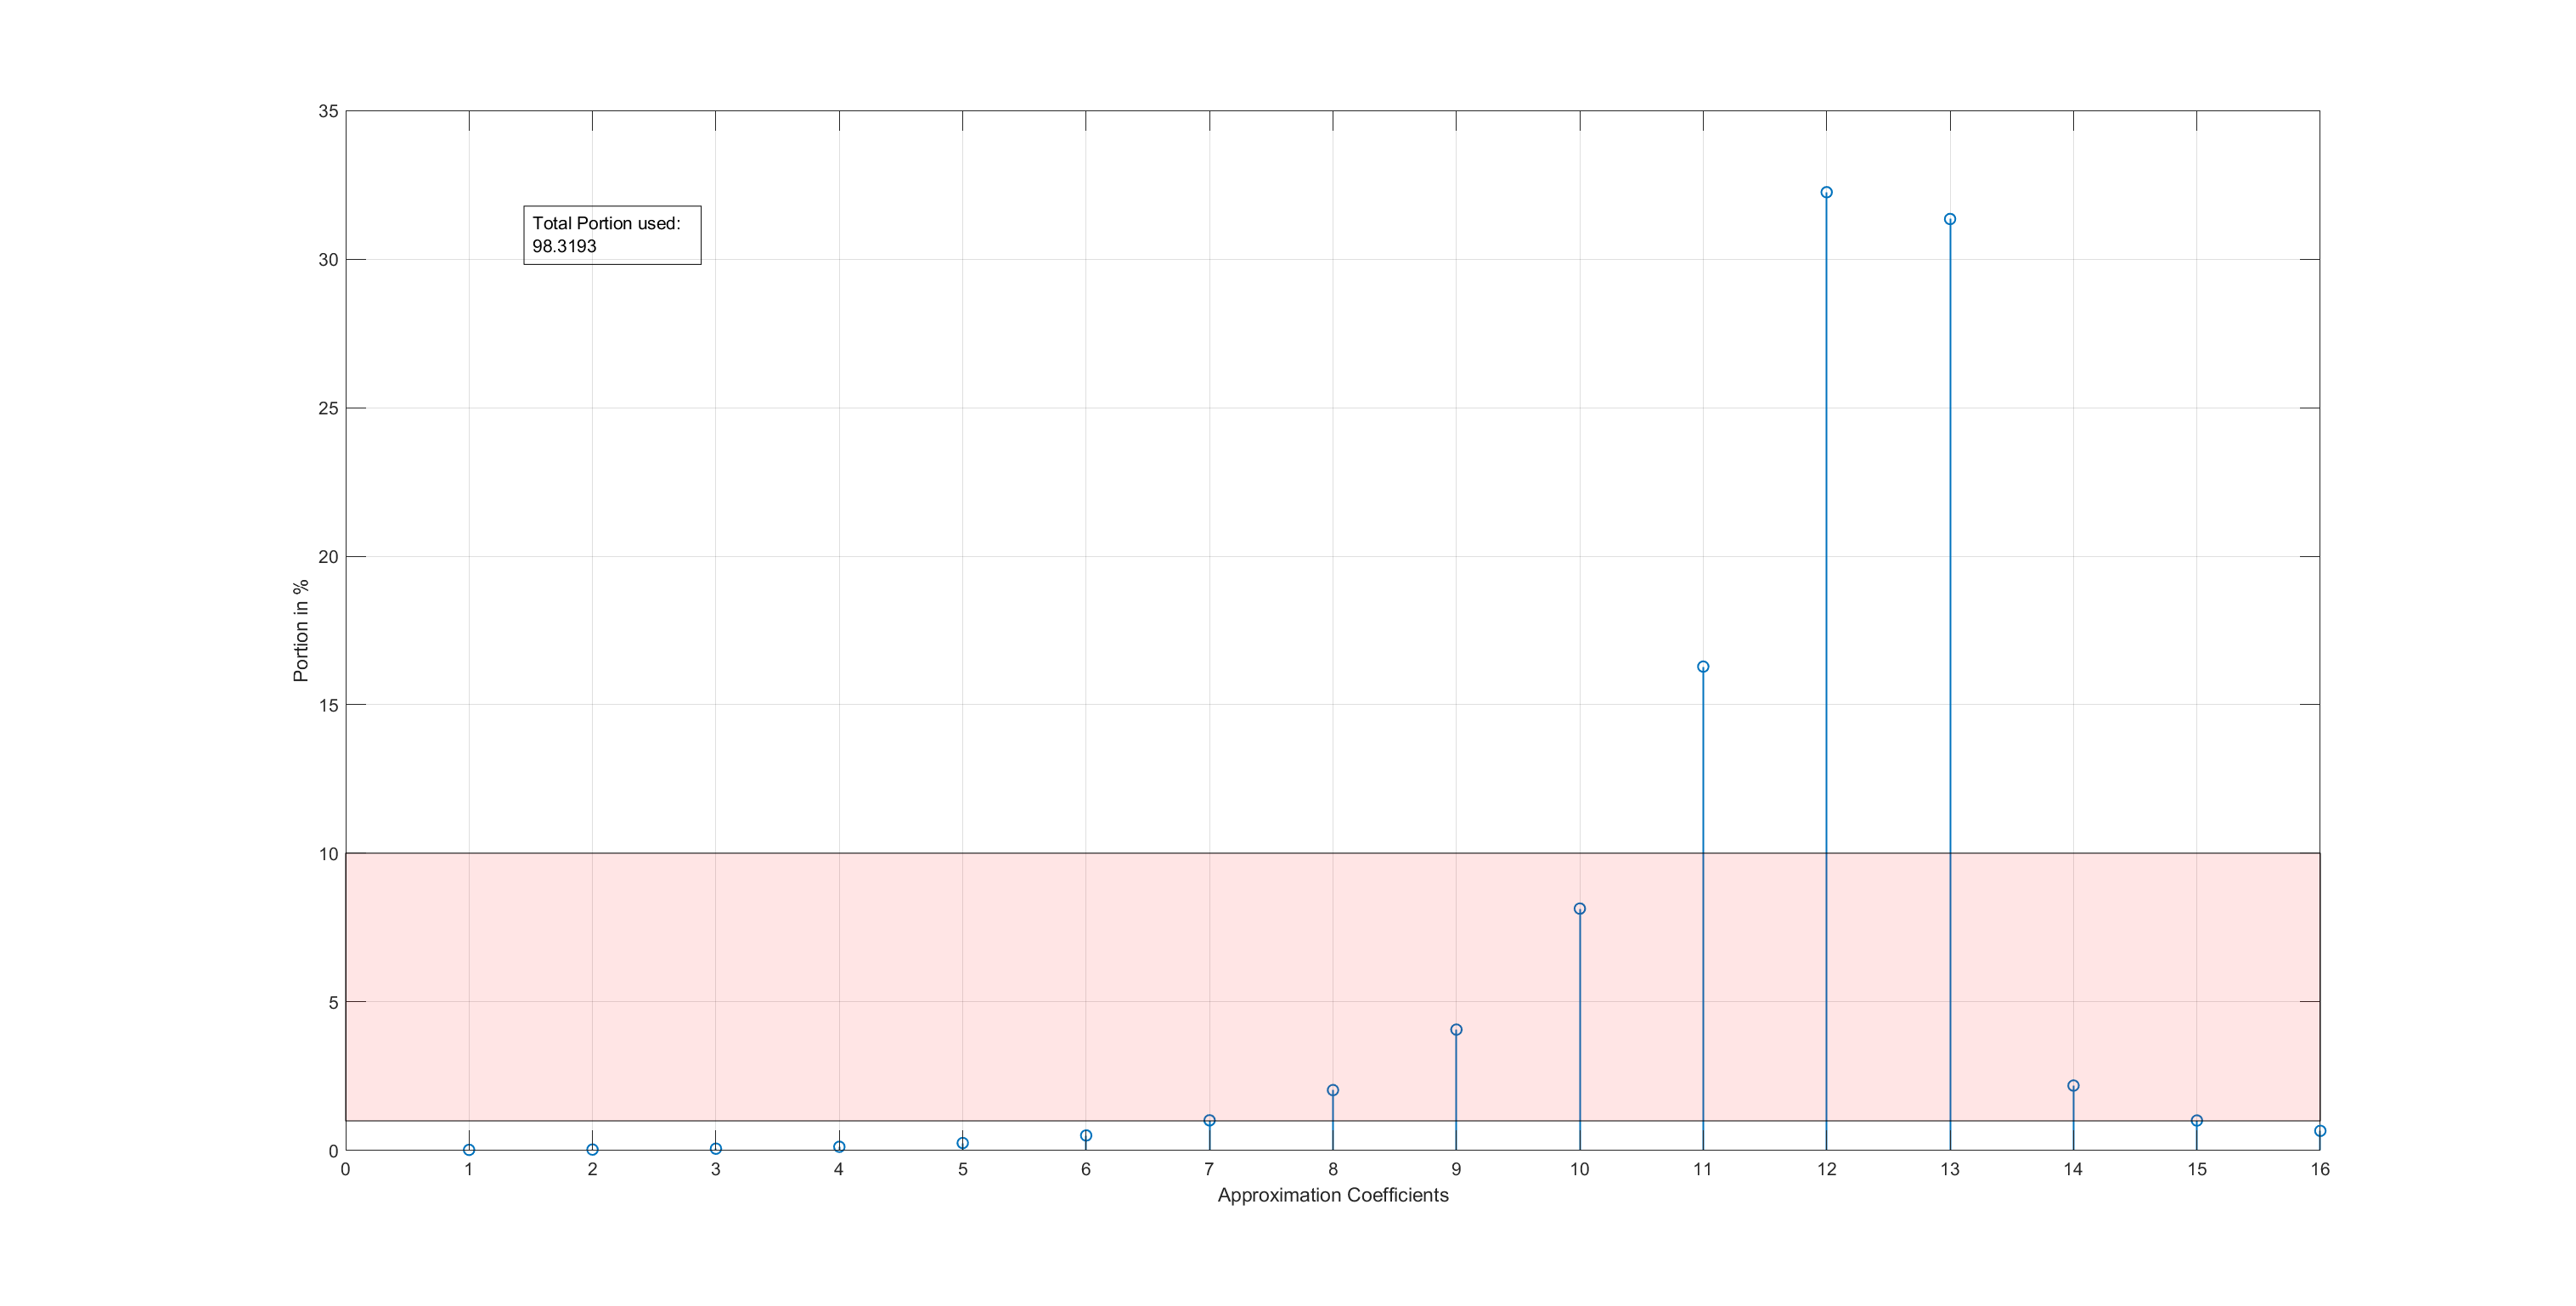
\includegraphics[width=\linewidth]{papers/compress/Bilder/recCoefs}
	\caption{Anteil der einzelnen Dilatationslevels am gesamten Signal (in Prozent) mit Quantisierungsschranke (rot).}
	\label{fig:coefficients}
\end{figure} 

Wenn anschliessend alle Dilatationslevels per Addition zusammengerechnet werden, kann das exakte Signal rekonstruiert werden.
Das Ziel ist jedoch, nur das nötige zu speichern.
Um das zu erreichen muss entschieden werden, ab wann es Sinn macht, die Werte zu speichern oder gegebenenfalls einzusparen.

\subsection{Erster Versuch}
Für einen ersten Versuch wird der Anteil der einzelnen Levels über das ganze Signal berechnet.
In \autoref{fig:coefficients} ist graphisch dargestellt, welchen Anteil vom originalen Signal die unterschiedlichen Dilatationen beinhalten.
Eine ungefähre Grössenanordnung lässt sich für einfache Signale wie in \autoref{fig:sawtooth} auch optisch einschätzen.
Signale mit breiten Bereichen einer hohen Amplitude resultieren auch in einem hohen Anteil am Gesamtsignal. 
Hingegen haben Signale, welche hauptsächlich Amplituden um den Nullpunkt herum besitzen einen eher geringen Einfluss auf das Signal.
Allerdings spielen die Anteile bei geringerer Dilatation insbesondere für Rauscheffekte trotzdem eine Rolle.

Im nächsten Schritt werden zwei Grenzen gesetzt.
Eine obere bei  $10\,\text{\%}$ und eine untere bei $1\,\text{\%}$ der Gesamtsignalstärke.
Diese `Schranke' unterteilt den Graphen nun in drei Bereiche. 
Oberhalb der Schranke sollen die exakten Werte übernommen werden, was beispielsweise bei CD-Qualität einer Genauigkeit von 16 Bit entspricht.
Unterhalb der Schranke können die Werte jedoch ganz weggelassen werden.
Der Bereich innerhalb der Schranke bildet einen Übergangsbereich.
Diese Werte sollen erhalten bleiben jedoch ist die Genauigkeit nicht vordergründig.

Beim Beispiel des Sägezahnes ist in \autoref{fig:coefficients} ersichtlich, dass die Levels 11, 12 und 13 exakt übernommen werden.
Hingegen werden die Levels 1 bis 6 sowie 16 weggelassen und die übrigen quantisiert.
Mit `Total Portion used' wird angegeben welcher Anteil des originalen Signals damit noch wiederhergestellt werden kann.

\subsection{Periodische Signale}
Als erstes stellt sich die Frage, ob diese Analyse für periodische Signale interessant ist.
Die Fouriertheorie (\autoref{chapter:fourier}) ermöglicht es einem, periodische Signale mit relativ wenigen harmonischen Schwingungen zu rekonstruieren.
Doch wie gut funktioniert es mit den hier verwendeten Daubechies-Wavelets?

\begin{figure}
	\centering
	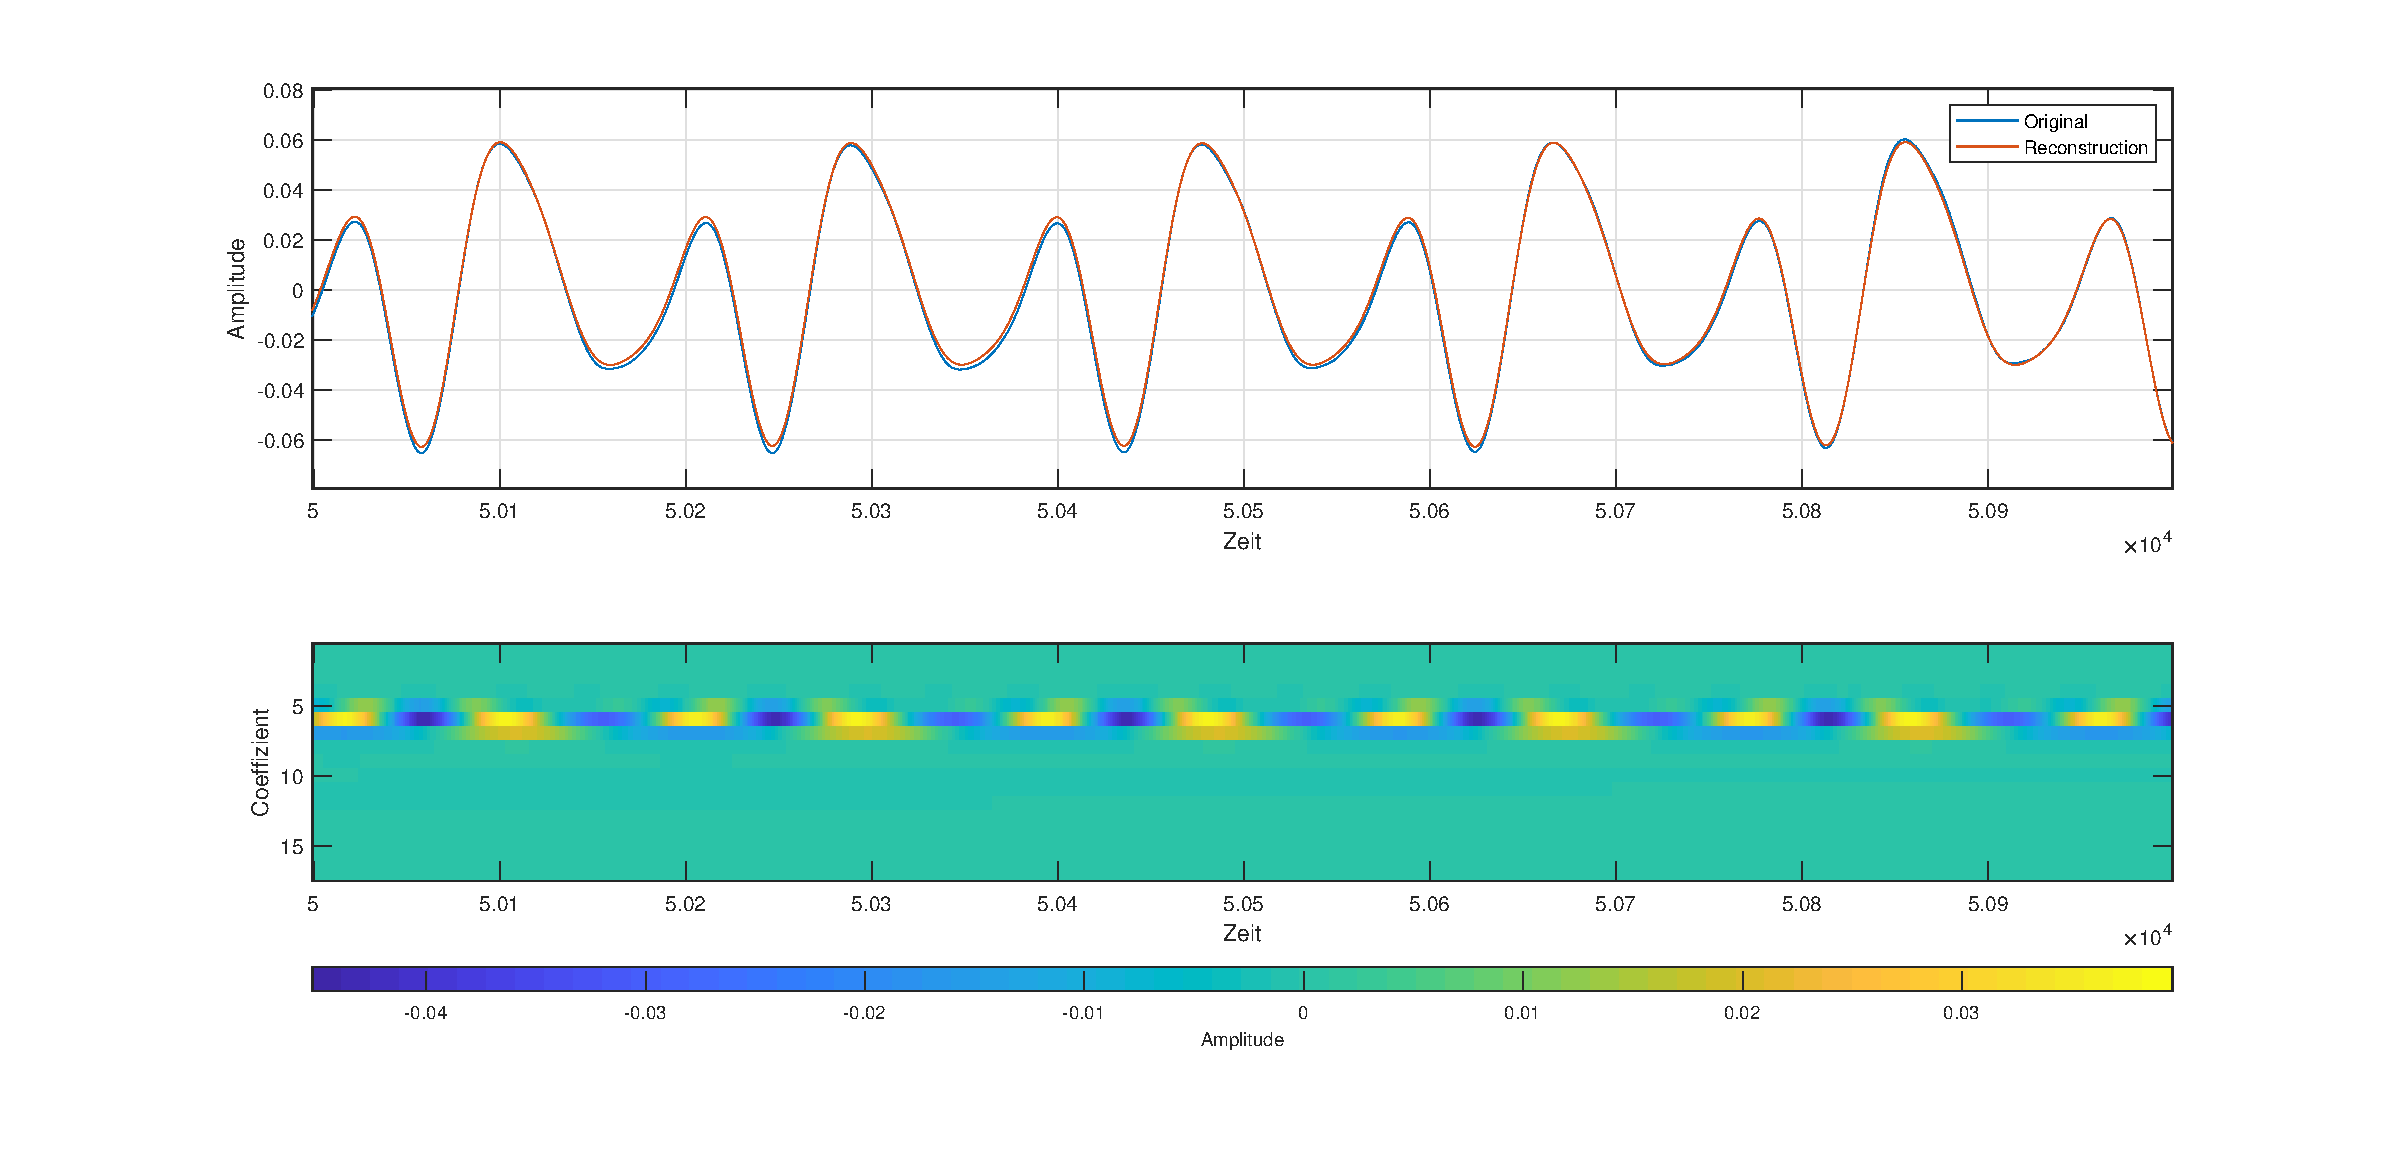
\includegraphics[width=\linewidth]{papers/compress/Bilder/frenchHorn_normal.pdf}
	\caption{Analyse eines Horntons mit dem Daubechies Wavelet db20.}
	\label{fig:horn}
\end{figure}

Als zweites Beispiel wird in \autoref{fig:horn} ein Horn-Ton untersucht.
Auch hier kann das periodische Signal mit wenigen Koeffizienten recht exakt beschrieben werden. 
Zum Vergleich sind in \autoref{fig:dbHorn} die Anteile der Levels mit einem db4 und einem db20 abgebildet.
\begin{figure}
	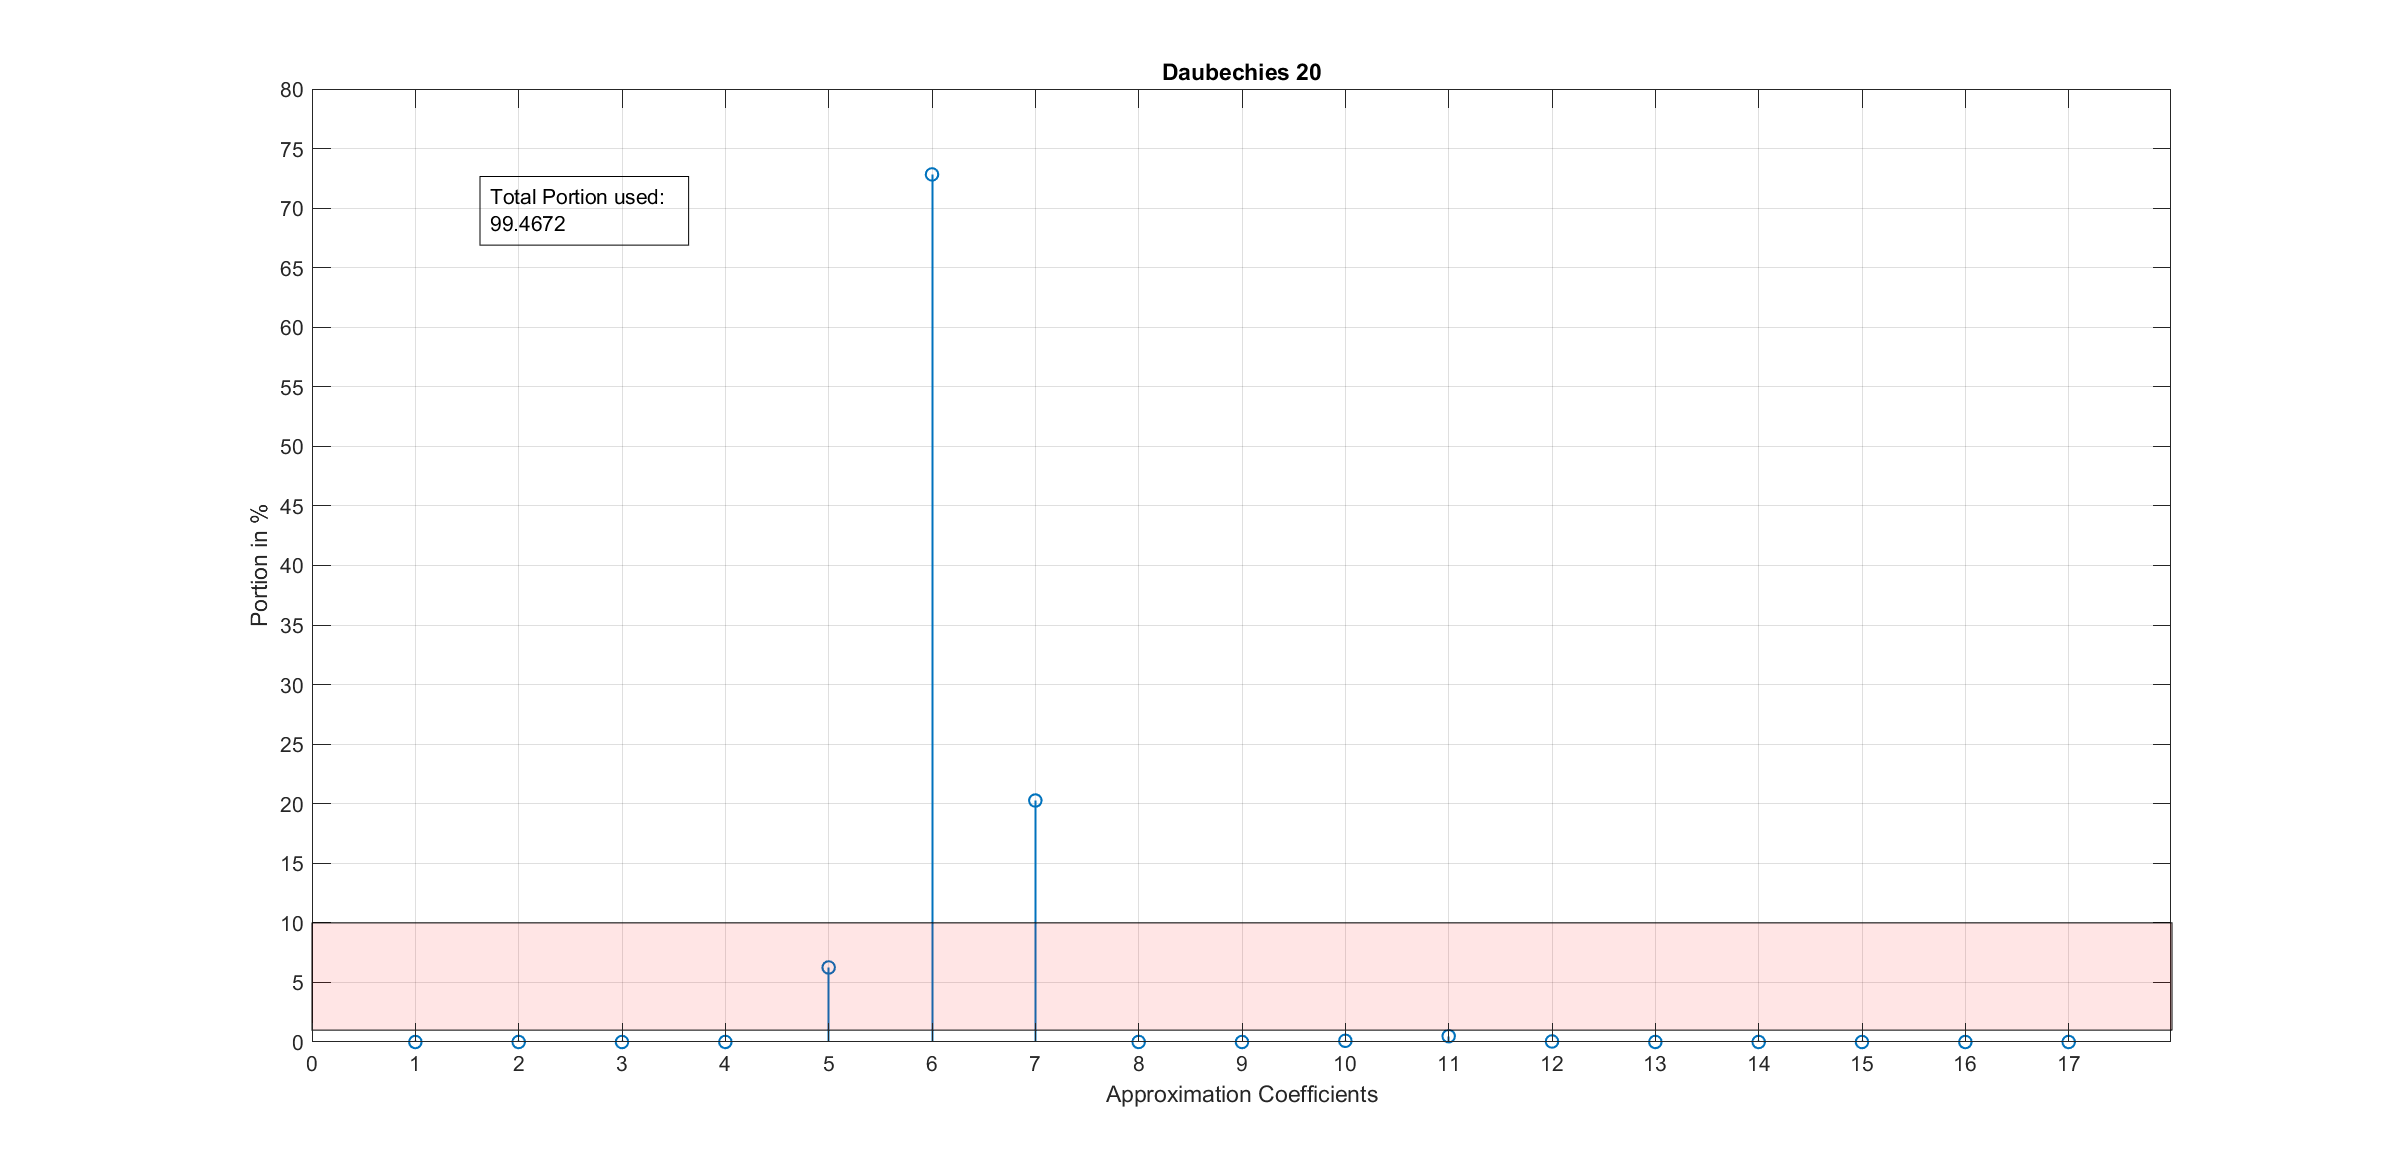
\includegraphics[width=0.5\linewidth]{papers/compress/Bilder/frenchHorn_db20.pdf}
	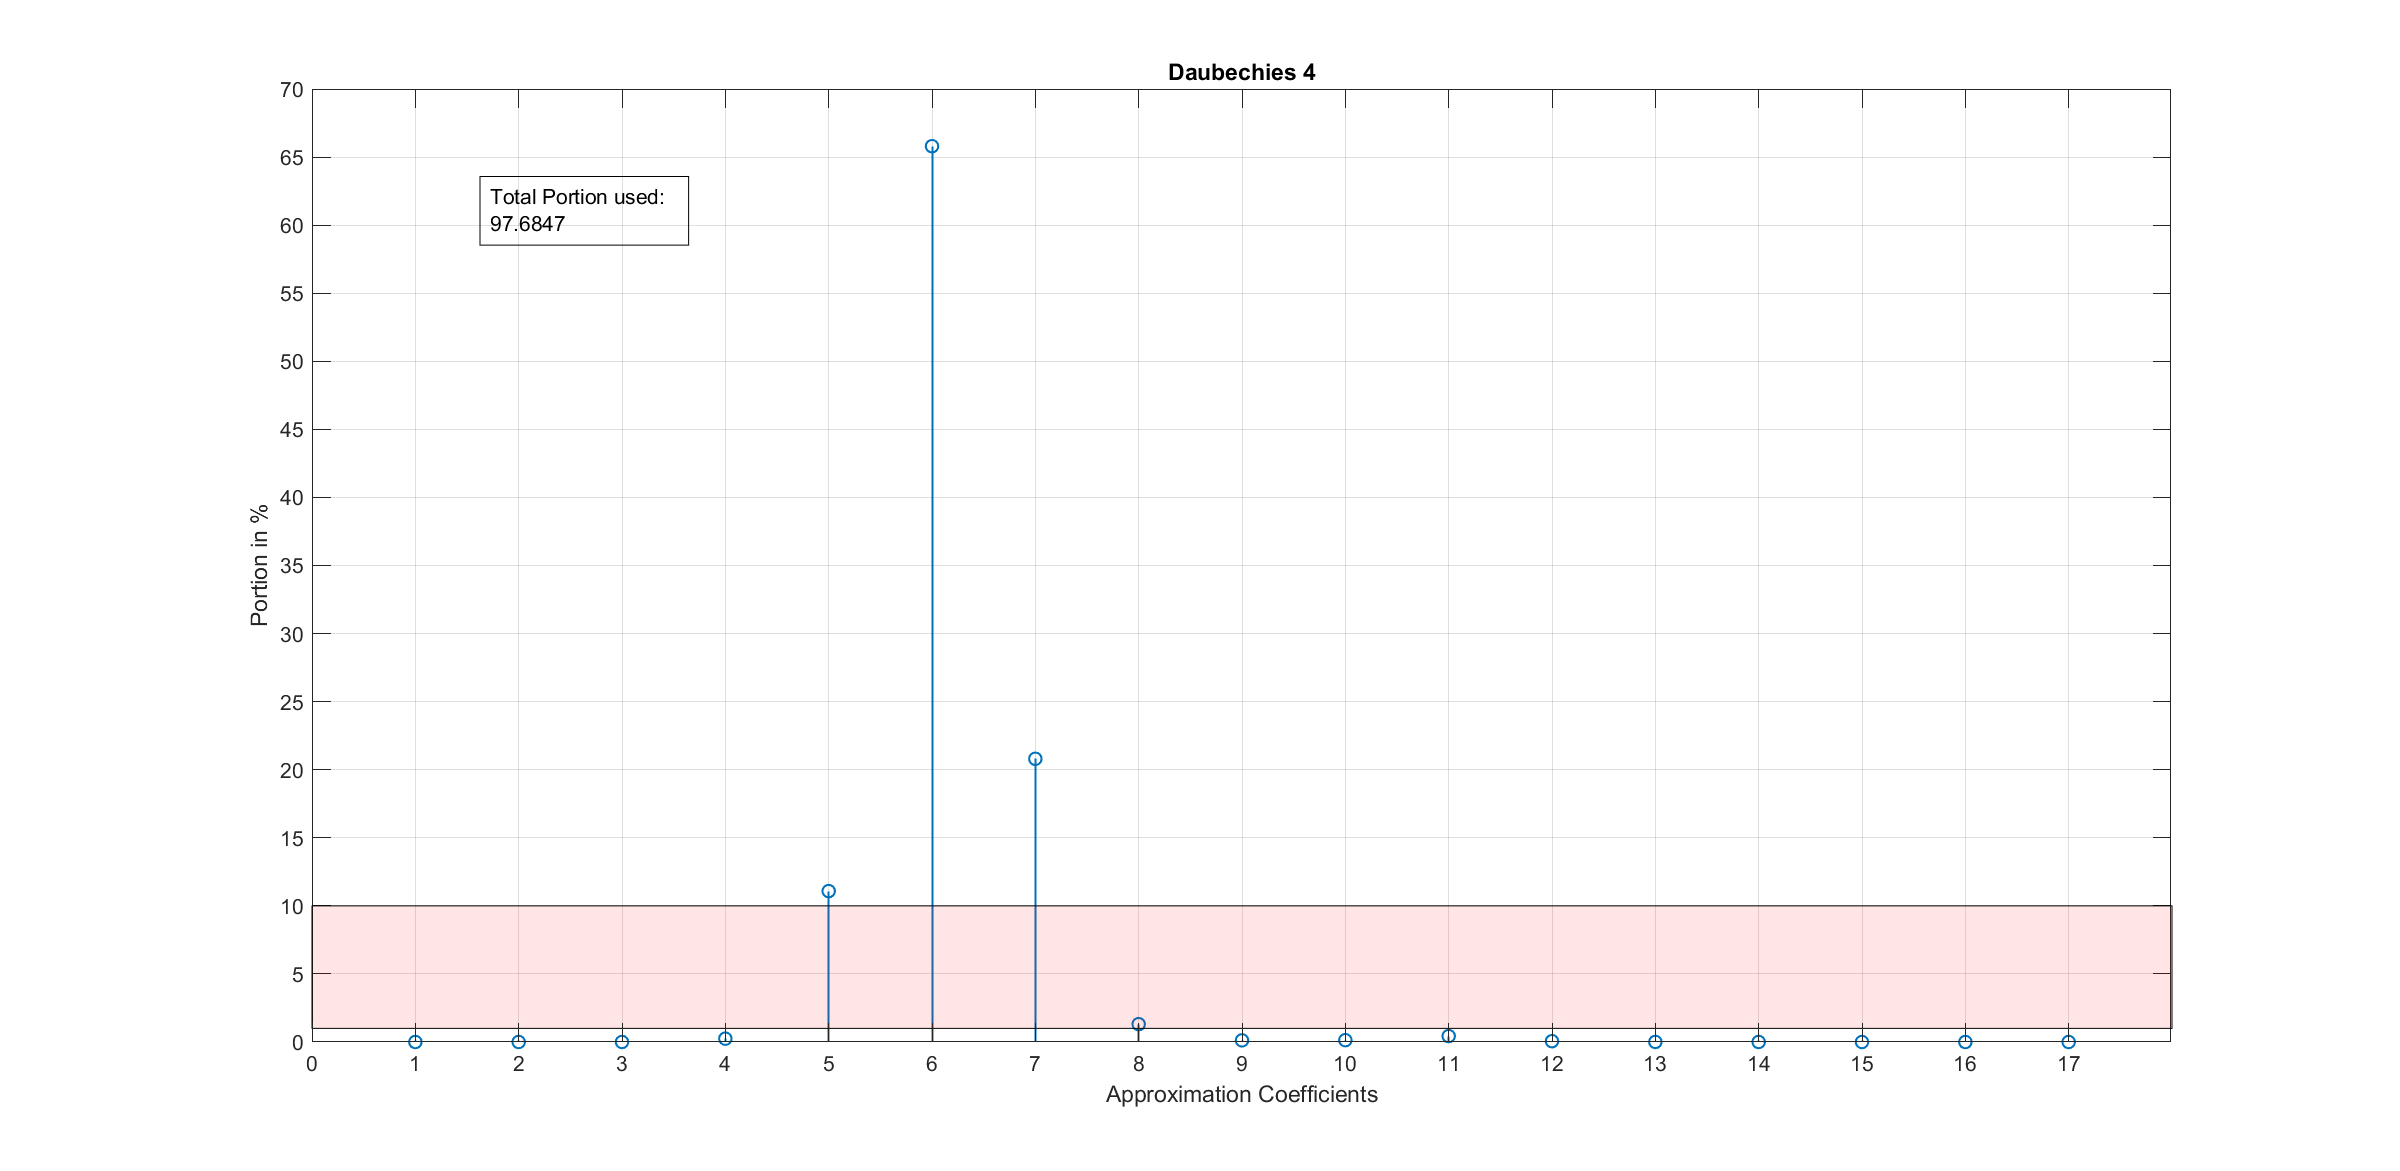
\includegraphics[width=0.5\linewidth]{papers/compress/Bilder/frenchHorn_db4.pdf}
	\caption{Anteil der verschiedenen Levels einer MSA an einem Hornton. Verwendet wurden Daubechies Wavelets der Ordnung vier und zwanzig.}
	\label{fig:dbHorn}
\end{figure}

Das Interessante ist nun, dass das harmonische Signal sehr gut mit dem db20 erfasst wird und über $99\,\text{\%}$ mit nur 3 Koeffizienten rekonstruiert werden kann.
Wird das Signal jedoch rekonstruiert zeigt sich ein grosses Problem der Quantisierung.
Das Signal wird teilweise stark verzerrt, was in \autoref{fig:hornBoth} gut ersichtlich ist.
Obwohl diese Verzerrungen anteilsmässig keinen grossen Unterschied zum Originalsignal machen, sind diese hochfrequenten Störungen akustisch sehr gut wahrnehmbar.

\begin{figure}
	\centering
	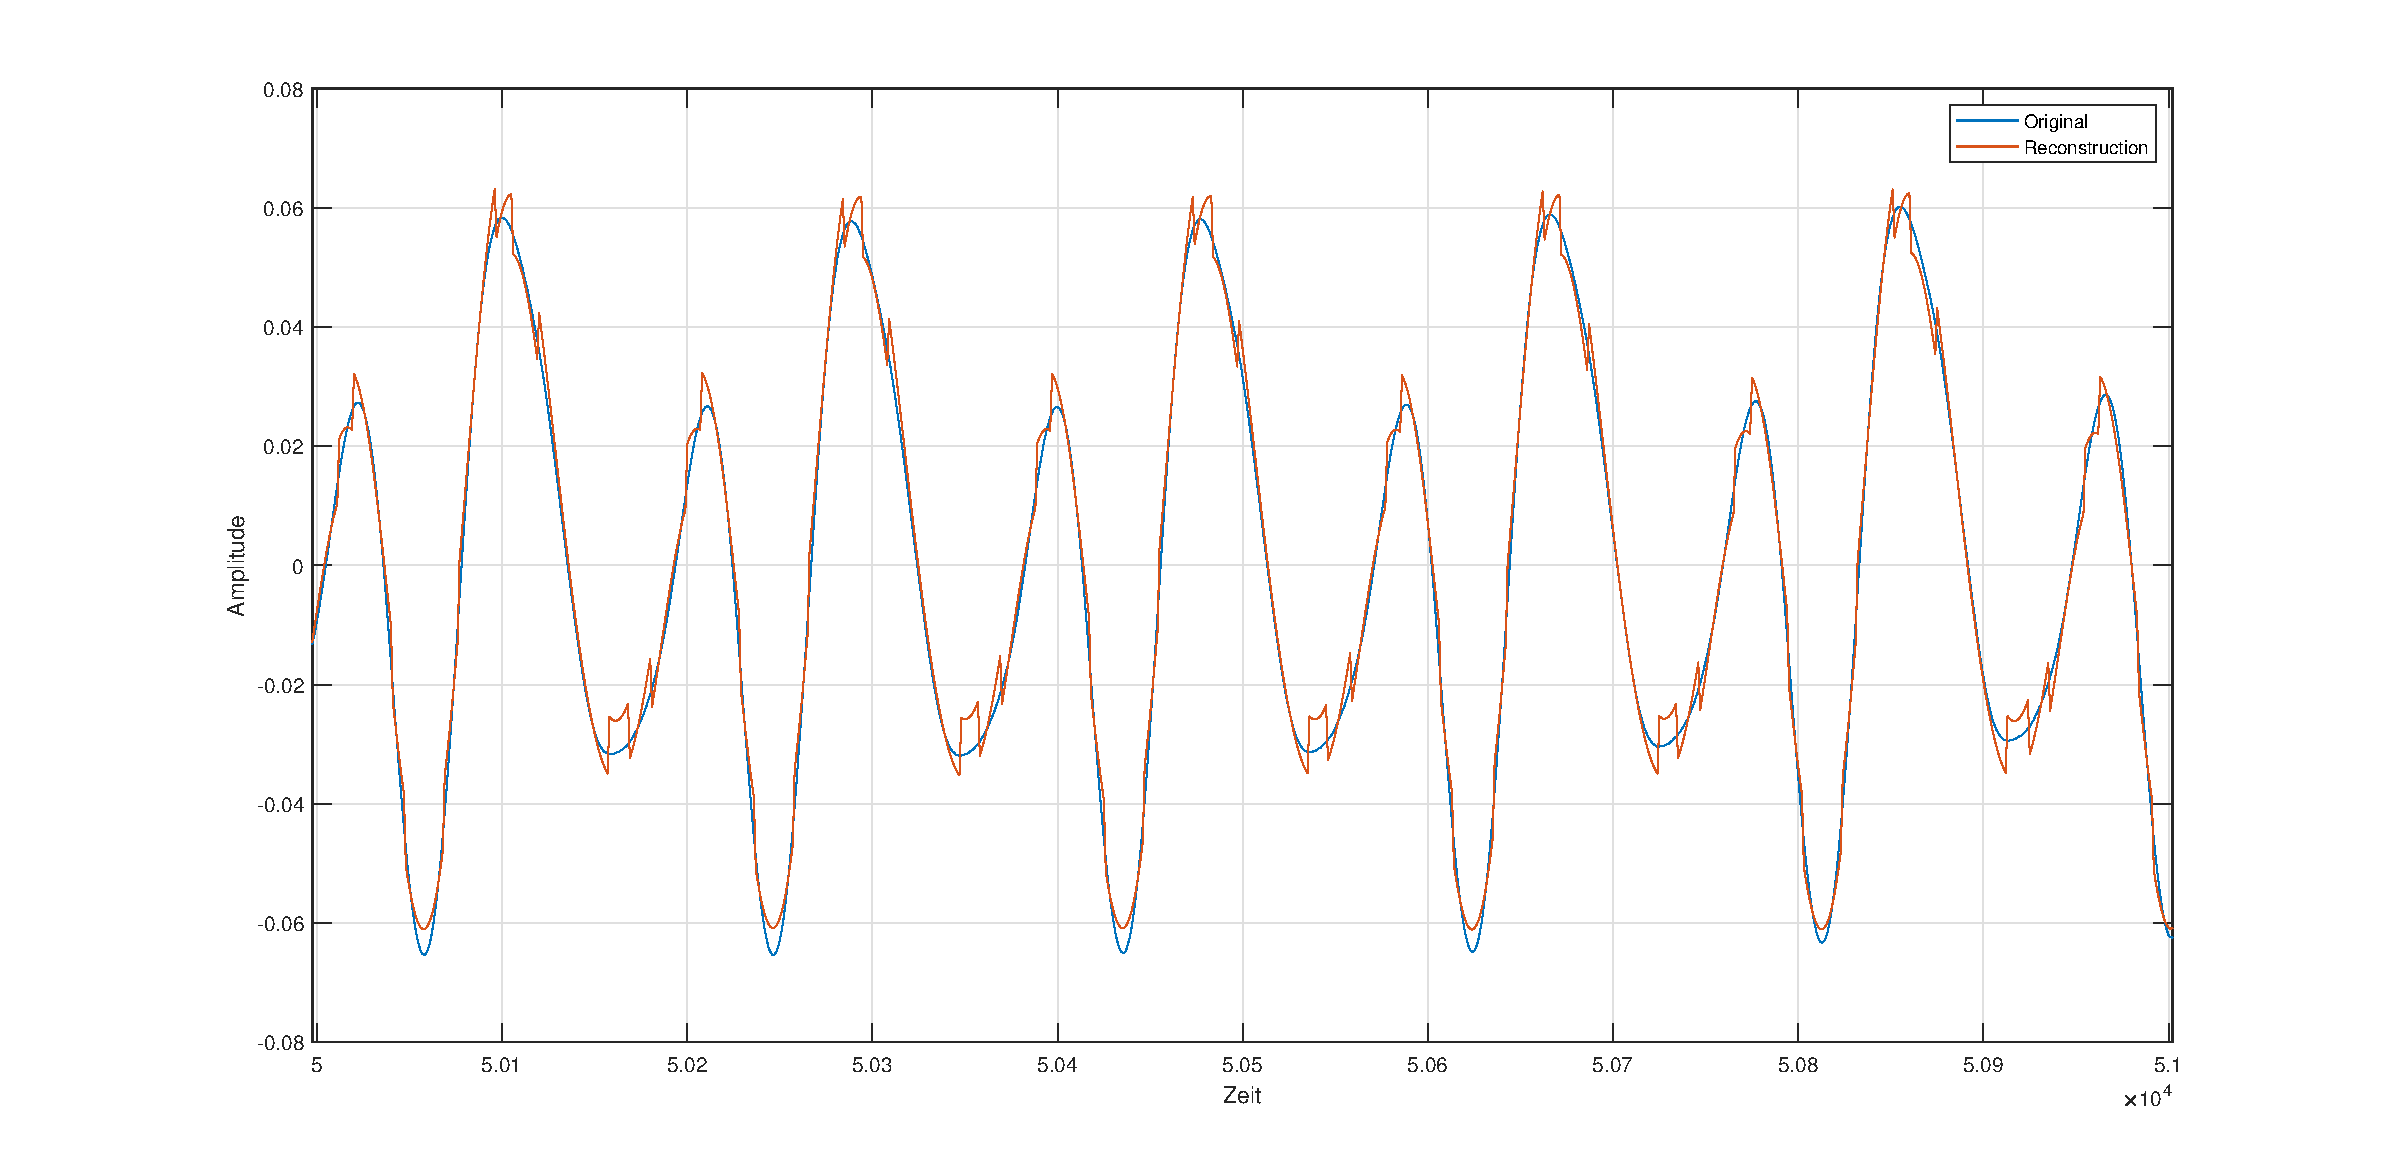
\includegraphics[width=\linewidth]{papers/compress/Bilder/hornBoth.pdf}
	\caption{Starke Verzerrungen des Horntons nach einer Rekonstruktion mit dem db20.}
	\label{fig:hornBoth}
\end{figure}

\begin{figure}
	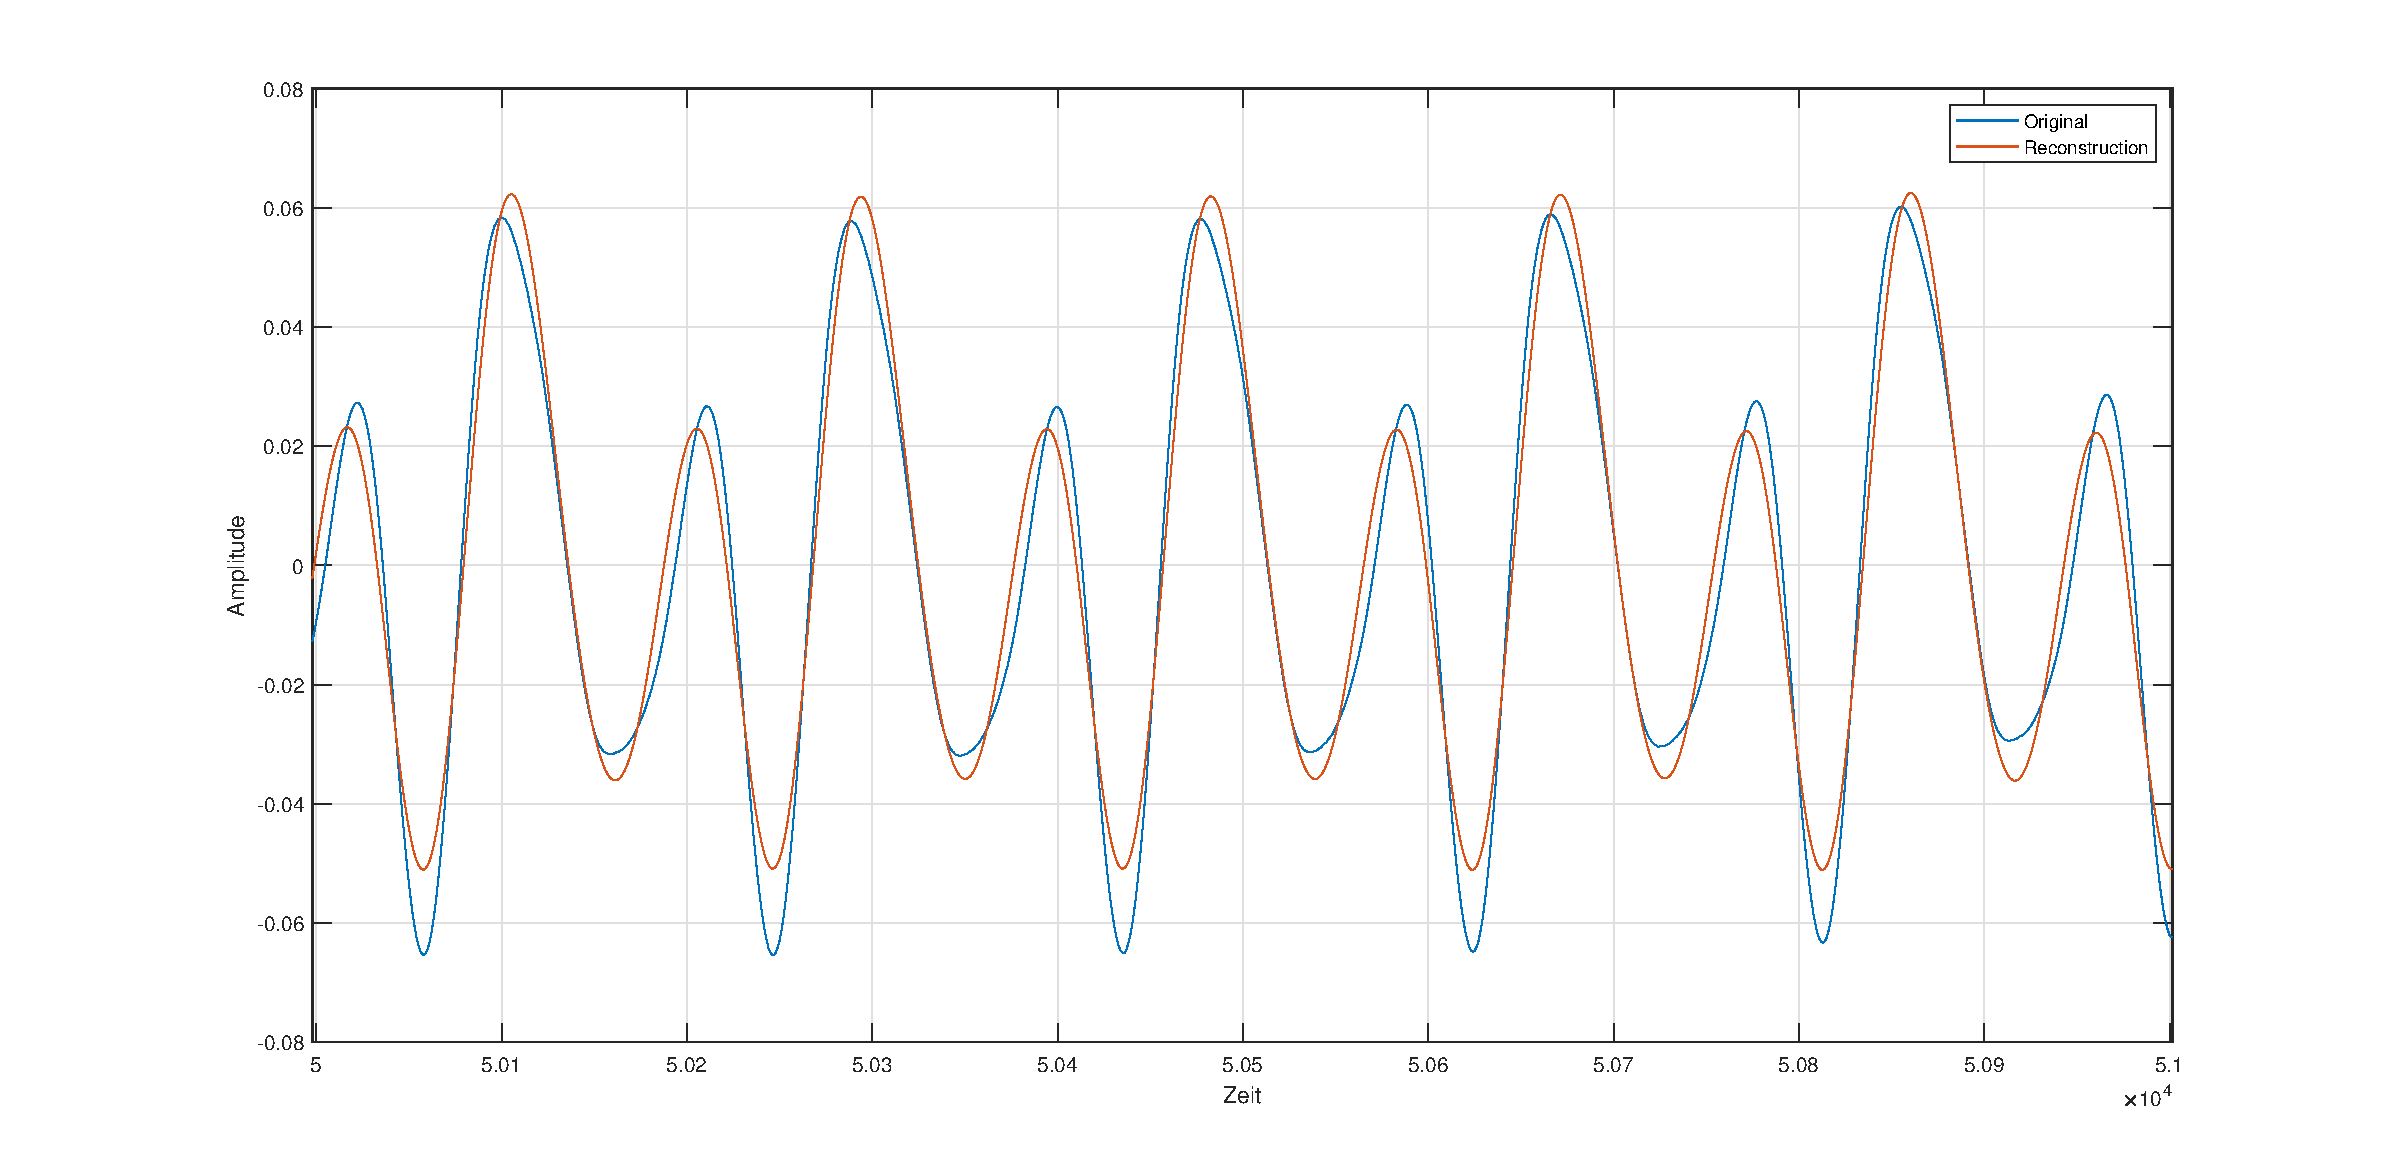
\includegraphics[width=0.5\linewidth]{papers/compress/Bilder/hornOnlyLevs.pdf}
	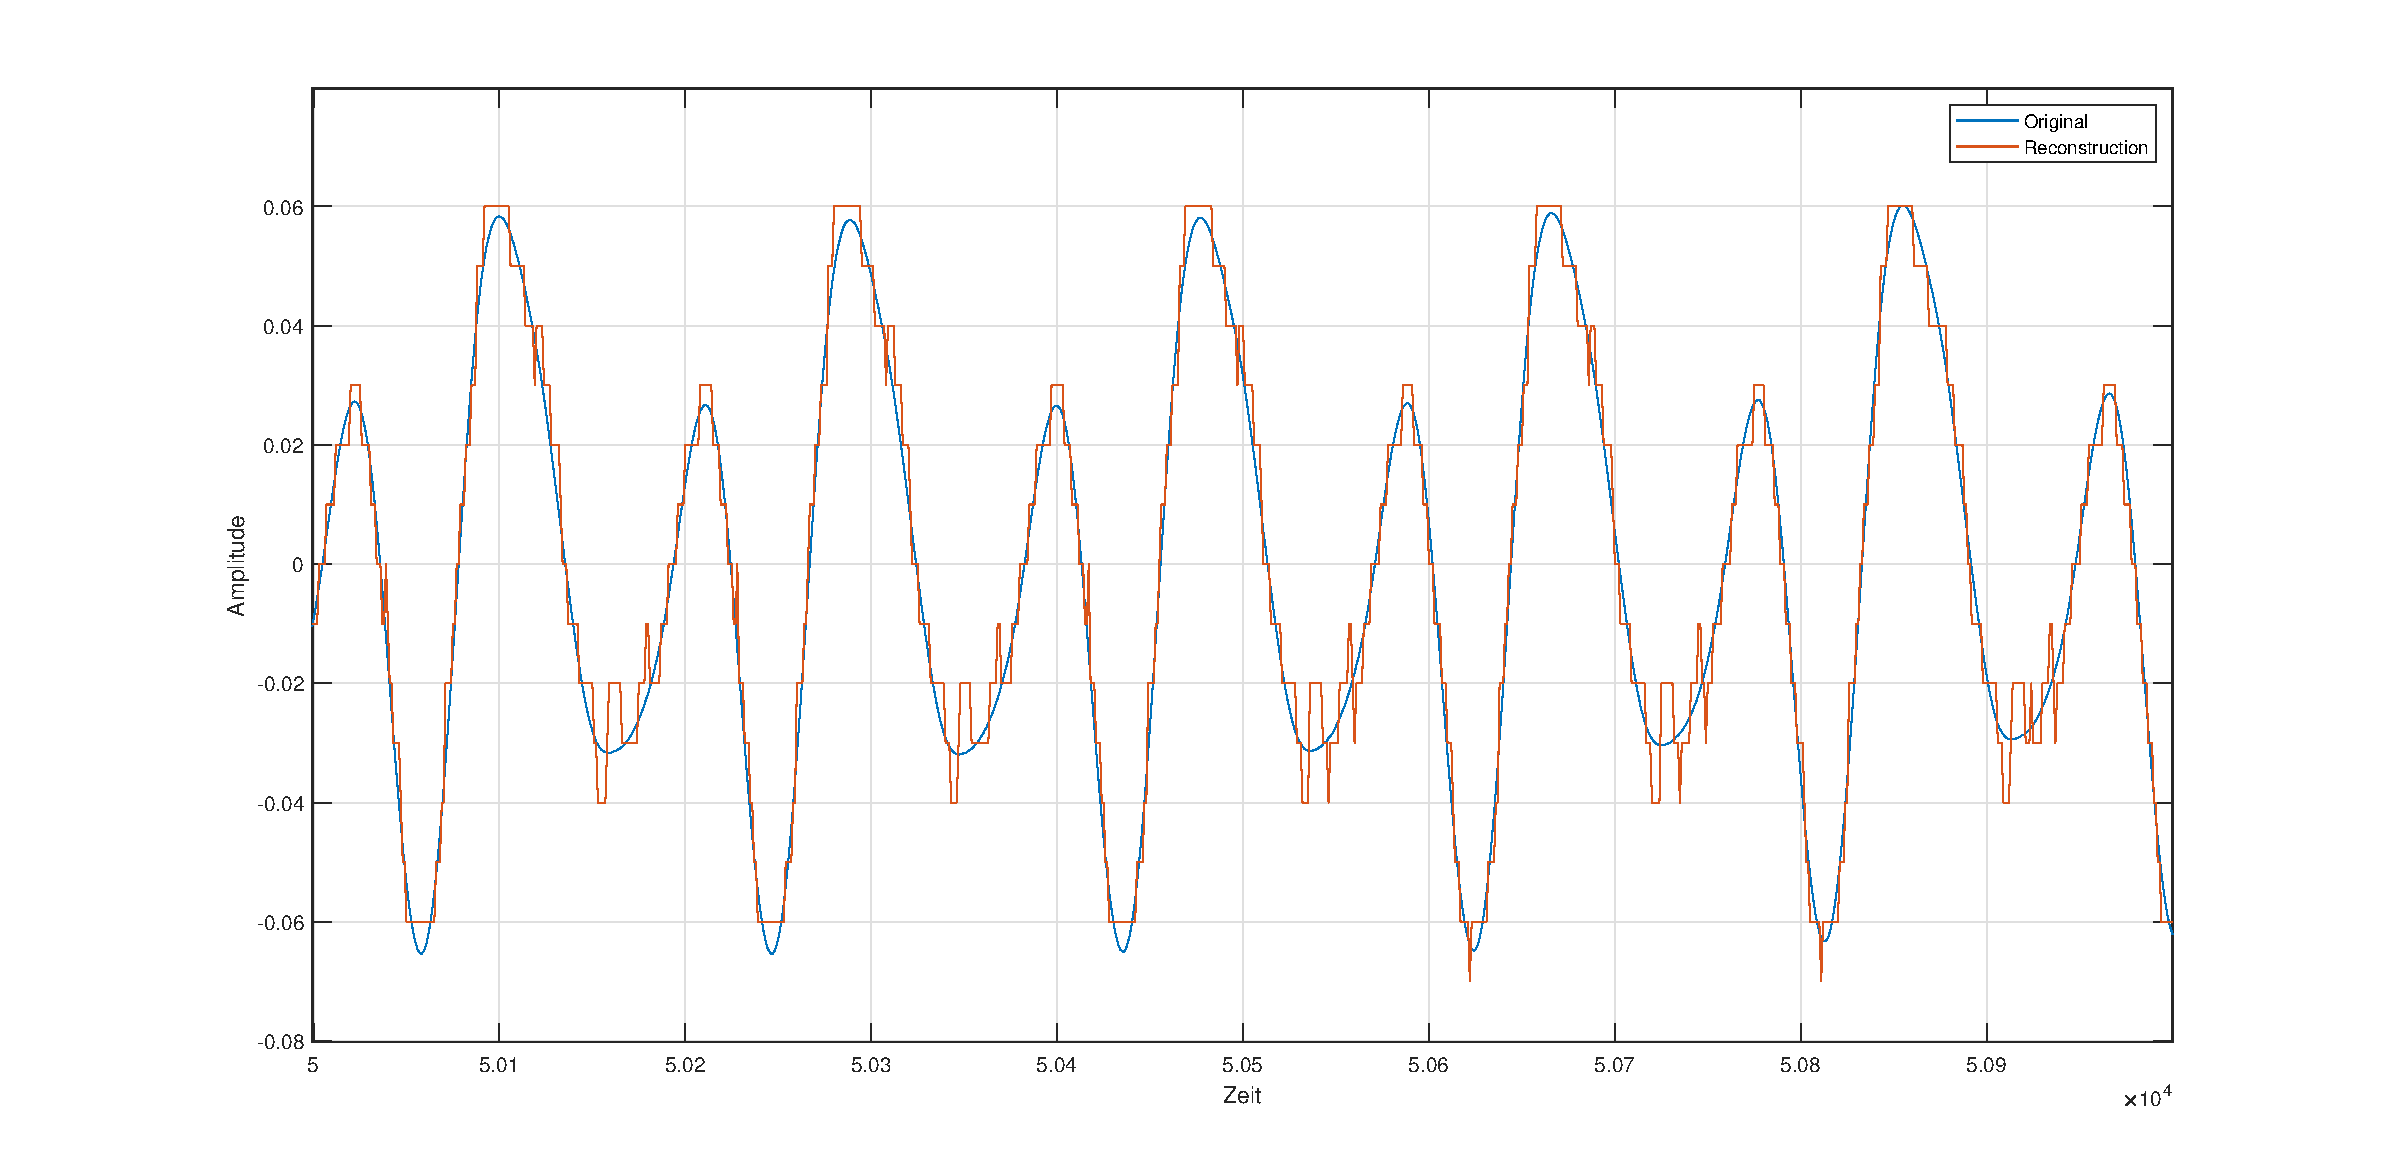
\includegraphics[width=0.5\linewidth]{papers/compress/Bilder/hornOnlyQuant.pdf}
	\caption{Das weglassen einiger Dilatationslevels resultiert nur in geringfügiger Änderung des Origiansignals(links).
		Eine Quantisierung über alle Dilatationslevels hat eine grosse Änderung des Ergebnisses zur Folge (rechts).}
	\label{fig:hornOnly}
\end{figure}
Um zu verstehen woher diese Störung kommt, wird die Rekonstruktion aufgeteilt.
In \autoref{fig:hornOnly} links werden alle Koeffizienten unterhalb der gesetzten Schranke verwendet. 
Das bedeutet, dass noch keine Quantisierung vorgenommen, sondern lediglich einen Teil der Koeffizienten weggelassen wird.
Dieses Signal weicht nur geringfügig vom Orignal ab.
Daraus lässt sich vermuten, dass das Problem an der Quantisierung liegt.
Wird die vollständige Rekonstruktion quantisiert, wird aus dem Originalsignal je nach gewählter Auflösung eine Treppenstufe wie sie in \autoref{fig:hornOnly} rechts zu sehen ist.
Bei der Analyse mit dem db4 wird das Signal zwar weniger exakt rekonstruiert, jedoch werden keine Levels quantisiert(\autoref{fig:dbHorn}).
Somit entstehen keine Verzerrungen und akustisch ist kaum ein Unterschied erkennbar.

Das zeigt zwei wesentliche Probleme.
Zum einen scheint es zu grob zu sein, über ein gesamtes Level zu entscheiden ob es quantisiert werden soll oder nicht.
Diese Einteilung soll deshalb auch innerhalb der einzelnen Levels gemacht werden, damit die Koeffizienten einzeln eingestuft werden können.
Zum anderen kann auch die Quantisierung nicht absolut gemacht werden.
Die Grösse des Anteils der Quantisierungsstufe wächst proportional mit der Grösse des Signals.
Es ist deshalb nötig, der Quantisierung besondere beachtung zu schenken.

\subsection{Quantisierung}
Audiodaten werden bei der CD-Qualität mit einer Auflösung von $16\,\text{Bit/Sample}$ abgespeichert. 
Bei einer Abtastfrequenz \textit{fs} von $44.1\,\text{kHz}$ heisst das, dass eine Datenrate \textit{d} von 
\begin{equation}
\textit{d} = \frac{\textit{n} \cdot \textit{fs}}{8\,\text{Bit/Byte}} = \frac{16\,\text{Bit/Sample} \cdot 44.1\,\text{kHz}}{8\,\text{Bit/Byte}} = 88.2\,\text{kB/s}
\end{equation}
resultiert.

Doch warum genau $16\,\text{Bit}$?
Nach \autoref{chapter:Psychoakustik} entspricht eine Verdoppelung des Signals gerade einer Erhöhung um $6\,\text{dB}$.
Bei einem Wertebereich von 16 Bit - wobei jedes zusätzliche Bit einer Verdoppelung des Wertebereichs entspricht - können Töne mit einer Lautstärke bis zu
$16\,\text{Bit}$ $\cdot$ $6\,\text{dB}$ = $96\,\text{dB}$
abgespeichert werden.
Je nach Tonspur ist aber so ein grosser Bereich nicht zwingend nötig.
Angenommen der Hornton erreicht maximal $80\,\text{dB}$, würden auch bereits ungefähr
$80\,\text{dB}$ / $6\,\text{dB}$ =  $13.3\,\text{Bit}$
genügen. 
Somit kann der Wertebereich der obersten $3\,\text{Bit}$ Bit weggelassen werden.

Zusätzlich wird wegen der Lautstärke von $80\,\text{dB}$ die Wahrnehmbarkeitsschwelle der orangen Kurve in \autoref{fig:Wahrnehmbarkeitsschwelle} um ungefähr $18\,\text{dB}$ angehoben.
Somit können auch die untersten $3\,\text{Bit}$ weggelassen werden.
Der Speicherbedarf hat sich also bereits von $16\,\text{Bit}$ auf $10\,\text{Bit}$ gekürzt, ohne dass ein markanter Unterschied hörbar ist.

Zusätzlich wird durch die Multiskalenanalyse das Sparpotential weiter vergrössert.
An Stellen mit hoher Amplitude (stark blau/gelb) sind genaue Werte wichtig.
Hingegen bei den Stellen mit tiefen Amplituden (türkis) wird diese Genauigkeit nicht gefordert und es genügt, die Koeffizienten quantisiert zu speichern.
Der Speicherbedarf der bereits reduzierten $10\,\text{Bit}$ kann noch um 2 weitere auf $8\,\text{Bit}$ verringert werden.
Die Datenrate entspricht demnach noch der Hälfte, $44.1\,\text{kB/s}$.
Es kann also für jeden Koeffizient bei dem ein Byte Genauigkeit ausreichend ist ein weiteres Byte gespart werden.

Wie häufig eine solche Einsparung möglich ist, hängt offensichtlich vom Signal ab.
Dieses Ergebnis weist aber erstaunliche Ersparnisse auf.
Können beispielsweise bei einem Drittel der Koeffizienten jeweils die Hälfte (1 Byte) gespart werden, benötigt es lediglich noch 5/6 vom Speicherplatz.

\subsection{Transiente Signale}
Da im Audiobereich nicht nur harmonische Komponenten vorhanden sind soll diese Analyse auch auf transiente Signale angewendet werden.
Dabei soll auch wieder die Auswirkungen einer Quantisierung überprüft werden.
Als Signal wird der Ruf eines Vogels, dem Wendehals (\textit{Jynx torquilla}), verwendet.
Der Wendehals hat einen sehr charakterischen Ruf mit steilen Übergängen.
\begin{figure}
	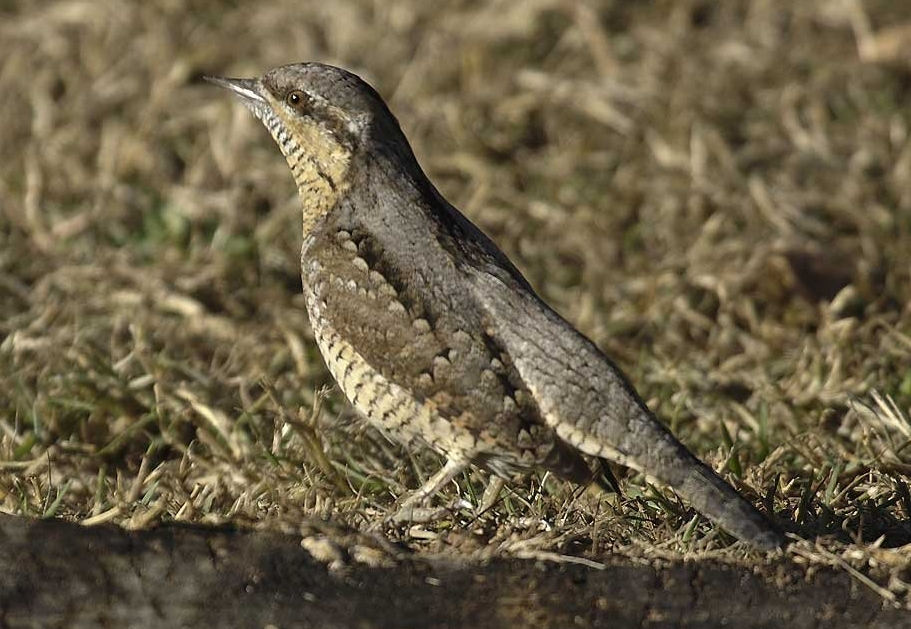
\includegraphics[width=0.4\linewidth]{papers/compress/Bilder/wendehals.jpg}
	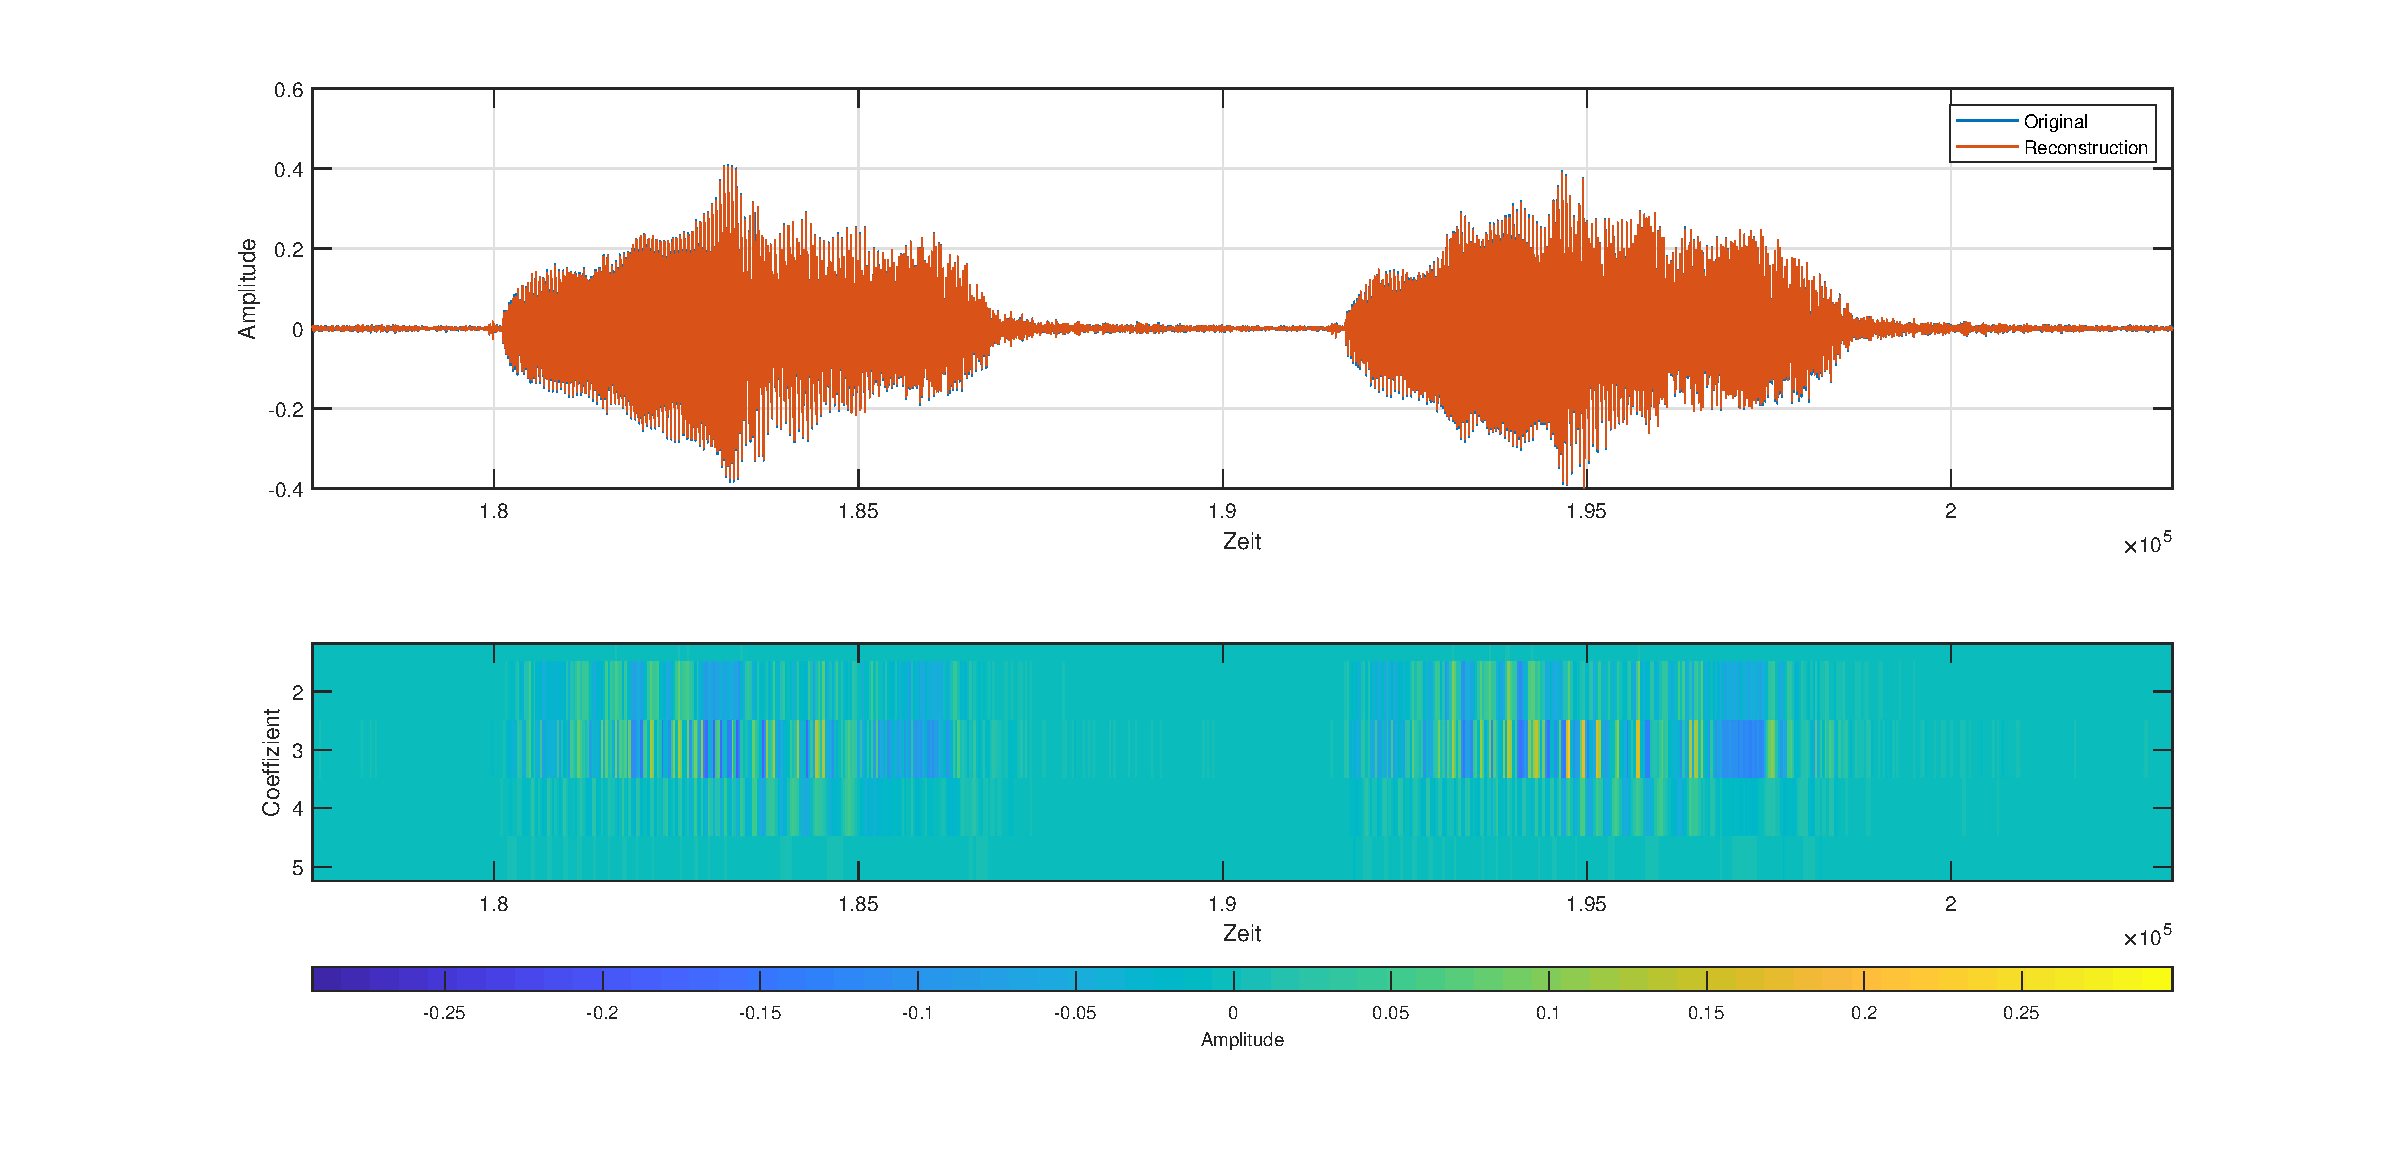
\includegraphics[width=0.6\linewidth]{papers/compress/Bilder/jynxAll.pdf}
	\caption{Der Wendehals (\textit{Jynx torquilla}) \cite{wikipedia:wendehals} mit seinem charakteristischen Ruf und der MSA.}
	\label{fig:jynxAll}
\end{figure}

Wie auch beim vorangehenden Beispiel ist der grösste Signalanteil in wenigen Koeffizienten der Multiskalenanalyse enthalten.
Durch die transienten Signale ist jedoch auch in den wichtigen Dilatationslevels eine ausgeprägte Magnitude vorhanden.
In \autoref{chapter:daubechies} wurde erklärt, dass mit den Daubechies-Wavelets Signale von gleicher und auch höherer Ordnung, wie das Wavelet selber erkannt werden können. 
Experimentell hat sich gezeigt, dass mit Wavelets einer höheren Ordnung eine bessere Rekonstruktion erreicht wird als mit den tiefen.
Das bedeutet aber nicht zwingend, dass die höheren auch besser geeignet sind.
Jedoch sind bei den tieferen Dilatationslevels die Wavelets breiter verteilt als bei den hohen und somit ist die Wahrscheinlichkeit grösser, dass ein Koeffizient quantisiert oder gelöscht wird. 
\begin{figure}
	\centering
	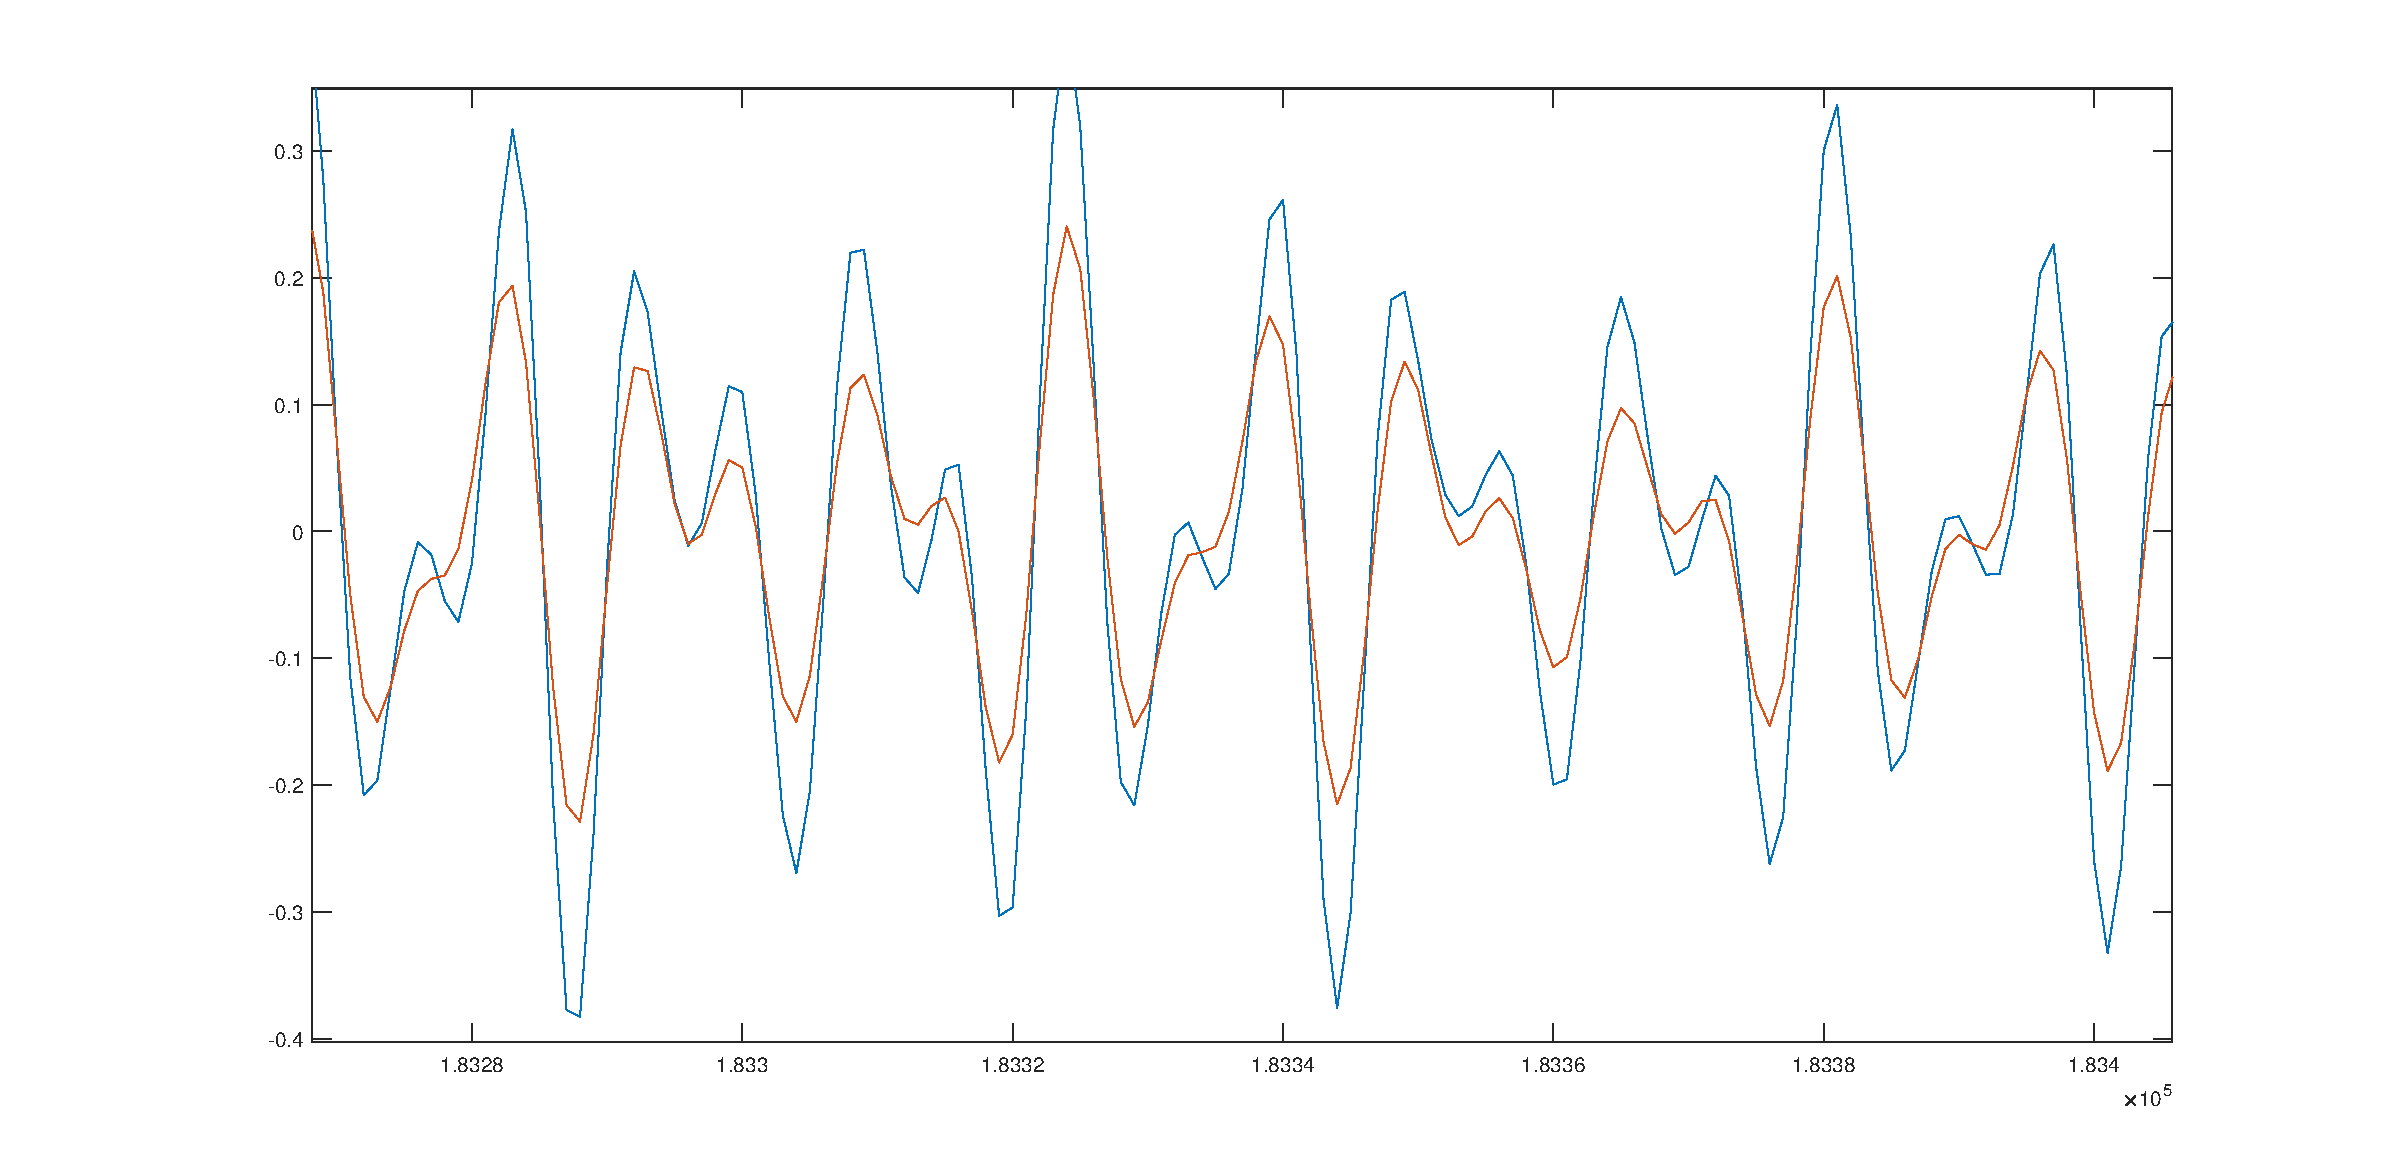
\includegraphics[width=\linewidth]{papers/compress/Bilder/jynxNear.pdf}
	\caption{Rekonstruktion des Vogelrufs, bei der nur das 6. Dilatationslevel verwendet wurde, welches ungefährt $75\,\textbf{\%}$ des Signals enthält.}
	\label{fig:jynx6}
\end{figure}
Es ist besonders erstaunlich, dass mit einem db20 Wavelet fast $75\,\text{\%}$ des gesamten Signals nur im 6. Level vorhanden ist.
In \autoref{fig:jynx6} ist eine Rekonstruktion zu sehen, bei welcher ausschliesslich dieses Level verwendet wird.
Akustisch ist der Klang des Wendehals immernoch gut erkennbar, jedoch ist die Energie und somit die Lautstärke des Signals niedriger.

\section{Schlussfolgerung}
\rhead{Schlussfolgerung}
Das Ziel dieser Arbeit war es, Erkenntnisse zur Audiokomprimierung mit Wavelets zu erhalten.
Wie sich herausstellt, ist es mit relativ geringem Aufwand möglich, eine Multiskalenanalyse mit numerischen Programmen wie MATLAB durchzuführen.
Die Beispiele haben gezeigt, dass die Gruppierung in wichtige, unwichtige und zu quantisierende Koeffizienten zu grob gemacht wurde. 
Zum einen kann kaum für all die unterschiedlichen Signaltypen im Audiobereich die selbe Grenze verwendet werden. 
Zum anderen sollte diese Analyse auch auf der Zeitachse unterteilt werden und somit eine dynamischere Einteilung ermöglichen. 
Die Arbeit hat jedoch mit einfachen Beispielen gezeigt, dass sich Wavelets gut eignen, um solche Signale zu erfassen.
Harmonische und auch transiente Signale wurden beide mit wenigen Levels genau dargestellt.
Besondere Vorsicht soll der Quantisierung der Koeffizienten geboten werden, da sie bei gewissen Signalen zu einer erheblichen verschlechterung des Hörerlebnis führen können.
In einem nächsten Schritt müsste von den erhaltenen Koeffizienten ausgehend ein passendes Audio-Format erstellt werden.

\printbibliography[heading=subbibliography]
\end{refsection}
